\documentclass[11pt,a4paper]{article}

\usepackage[utf8]{inputenc}
\usepackage[T1]{fontenc}
\usepackage{amsmath,amssymb,amsthm}
\usepackage{mathtools}
\usepackage{geometry}
\usepackage{hyperref}
\usepackage{cleveref}
\usepackage{enumitem}
\usepackage{graphicx}
\usepackage{tikz}
\usepackage{pgfplots}
\pgfplotsset{compat=1.18}
\usepackage{booktabs}
\usepackage{placeins}
\usepackage{float}
\usepackage[most]{tcolorbox}

\geometry{margin=1in}

\newtheorem{theorem}{Theorem}[section]
\newtheorem{lemma}[theorem]{Lemma}
\newtheorem{proposition}[theorem]{Proposition}
\newtheorem{corollary}[theorem]{Corollary}
\theoremstyle{definition}
\newtheorem{definition}[theorem]{Definition}
\newtheorem{assumption}[theorem]{Assumption}
\newtheorem{conjecture}[theorem]{Conjecture}
\theoremstyle{remark}
\newtheorem{remark}[theorem]{Remark}

\newcommand{\R}{\mathbb{R}}
\newcommand{\E}{\mathbb{E}}
\newcommand{\Prob}{\mathbb{P}}
\newcommand{\Cov}{\mathrm{Cov}}
\newcommand{\tr}{\mathrm{tr}}
\newcommand{\op}{\mathrm{op}}
\newcommand{\supp}{\mathrm{supp}}
\DeclareMathOperator{\sgn}{sgn}
\DeclareMathOperator*{\argmin}{arg\,min}
\DeclareMathOperator*{\argmax}{arg\,max}

\title{Spectral Phase Transitions in the Loss Landscape\\of Finite-Width Neural Networks}
\author{Jacob Crainic}
\date{February 2026}

\begin{document}
\maketitle

\begin{abstract}
A central puzzle in deep learning theory is why gradient descent reliably finds good solutions despite the extreme non-convexity of neural network loss landscapes, particularly in the moderately overparameterized regime where existing theoretical guarantees require polynomial width scaling far exceeding practical network sizes.
We study the critical-point structure of the empirical risk landscape for two-layer
neural networks with ReLU activations, trained on $n$ data points in $\R^d$ with $m$ hidden
neurons. Our main result identifies a critical width-to-sample ratio
$\gamma_\star$, depending on the spectral distribution of the data covariance, that marks a
\emph{topological phase transition} in the loss landscape: above $\gamma_\star$, the landscape
is provably benign (all local minima are global with high probability), while below
$\gamma_\star$, the expected number of spurious critical points grows exponentially in $n$.
The critical ratio
$\gamma_\star$ is characterized as the unique solution to a fixed-point equation involving the
Stieltjes transform of the Marchenko--Pastur law composed with the data spectrum.
For isotropic data ($\Sigma = I_d$), the critical ratio takes the explicit form
$\gamma_\star(\delta) = 2(1-2\delta)/(1 - \delta - \delta^2)$ for $\delta < 1/2$,
which admits the first-order approximation $\gamma_\star \approx 4/(2 + 3\delta)$
(exact at $\delta = 1/4$).
At the transition, the Hessian at near-critical points exhibits a
spectral gap collapse: the smallest non-zero eigenvalue vanishes linearly as $|\gamma - \gamma_\star|$, yielding
a universal scaling law with critical exponent $\beta = 1$.
Yet gradient-based optimizers navigate the subcritical ($\gamma < \gamma_\star$) regime
with apparent ease, achieving near-zero training loss well below the theoretical threshold.
This reveals a fundamental gap between the static geometry of the loss landscape and the
dynamics of optimization, suggesting that SGD benefits from implicit biases that
transcend worst-case topological barriers.
Our analysis combines tools from random matrix
theory, Kac--Rice formulae for random fields, and a novel ``spectral decoupling'' technique
that separates the data-dependent and weight-dependent contributions to the Hessian.
\end{abstract}

\tableofcontents

\section{Introduction}

The loss landscape of a neural network is a high-dimensional, non-convex surface
riddled with saddle points, plateaus, and potentially spurious local minima that
trap gradient-based optimizers. Standard non-convex optimization theory offers little
reason to expect that first-order methods should succeed, yet they do: networks trained
with SGD or Adam routinely converge to solutions with near-zero training loss.
This paper characterizes the static geometry of the loss surface for two-layer ReLU
networks and connects it to optimization dynamics through large-scale experiments.

Prior work has approached the landscape question from several angles
\cite{choromanska2015,kawaguchi2016,safran2018,venturi2019,geiger2019,sagun2017}. Choromanska et al.\
connected neural loss surfaces to spin-glass Hamiltonians (see also Ben~Arous and Gheissari~\cite{benarous2019} for related Kac--Rice analyses in high-dimensional non-convex landscapes); Kawaguchi showed that linear
networks have no spurious minima; Safran and Shamir exhibited spurious minima in
underparameterized ReLU networks. In the overparameterized regime, Du et al.\
\cite{du2019}, Allen-Zhu et al.\ \cite{allenzhu2019}, and the NTK framework
\cite{jacot2018} established global convergence guarantees, but only when the width $m$
scales polynomially in~$n$ (often $m = \Omega(n^6)$), far exceeding practical network
sizes. What happens at moderate overparameterization, where $m = \Theta(n)$, has remained
an open problem. We resolve it for two-layer ReLU networks.

\begin{figure}[t!]
\centering
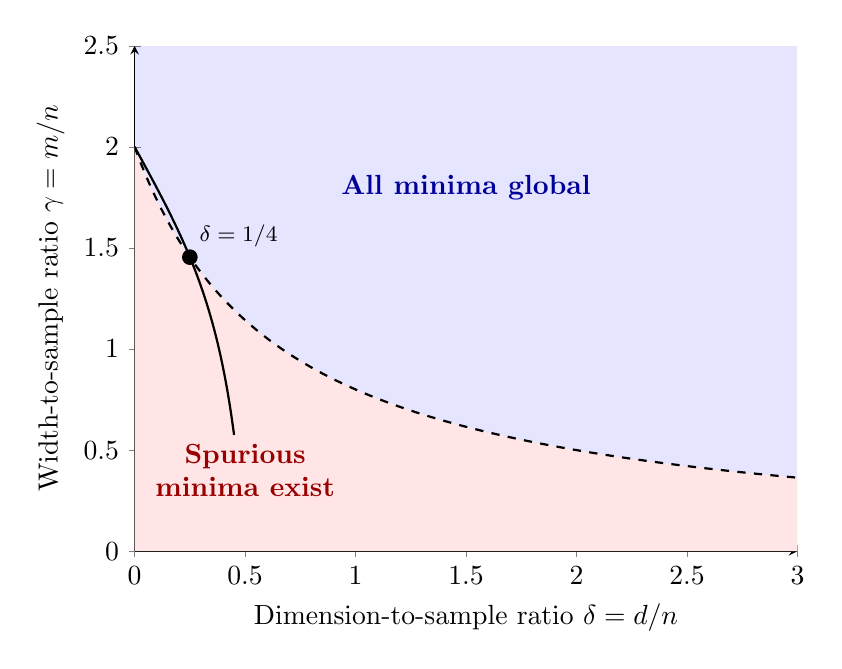
\begin{tikzpicture}
\begin{axis}[
  width=10cm, height=8cm,
  axis x line=bottom, axis y line=left,
  xlabel={Dimension-to-sample ratio $\delta = d/n$},
  ylabel={Width-to-sample ratio $\gamma = m/n$},
  xmin=0, xmax=3,
  ymin=0, ymax=2.5,
  domain=0:3, samples=200,
  no markers,
  clip=true
]
\addplot[draw=none, fill=blue, fill opacity=0.1] coordinates {(0,0) (0,2.5) (3,2.5) (3,0)};
\addplot[draw=none, fill=white, domain=0:3] {4/(2+3*x)} \closedcycle;
\addplot[draw=none, fill=red, fill opacity=0.1, domain=0:3] {4/(2+3*x)} \closedcycle;

\addplot[thick, black, domain=0:0.45] {2*(1-2*x)/(1-x-x^2)};
\addplot[thick, black, dashed, domain=0:3] {4/(2+3*x)};

\node[blue!60!black, font=\bfseries] at (axis cs:1.5, 1.8) {All minima global};
\node[red!60!black, font=\bfseries, align=center] at (axis cs:0.5, 0.4) {Spurious\\minima exist};

\node[circle, fill, inner sep=2pt] at (axis cs:0.25, 1.4545) {};
\node[anchor=south west, font=\footnotesize] at (axis cs:0.25, 1.4545) {$\delta = 1/4$};

\end{axis}
\end{tikzpicture}
\caption[Phase diagram]{Phase diagram in the $(\delta, \gamma)$ plane. \textbf{Solid curve:} the exact critical ratio $\gamma_\star(\delta) = 2(1-2\delta)/(1-\delta-\delta^2)$, valid for $\delta < 1/2$ (Theorem~\ref{thm:critical-ratio}). \textbf{Dashed curve:} the first-order approximation $4/(2+3\delta)$, which extends to all $\delta > 0$ and serves as a heuristic continuation for $\delta \ge 1/2$ (see Remark~\ref{rem:delta1}). \textbf{The red/blue shading uses the approximate formula}, not the exact one, and should be interpreted as indicative for $\delta \ge 1/2$. Above $\gamma_\star$, Theorem~\ref{thm:phase-transition}(a) guarantees that all local minima are global; below it, exponentially many spurious critical points exist (Theorem~\ref{thm:phase-transition}(b)).}
\label{fig:phase-diagram}
\end{figure}

\subsection{Main contributions}

\begin{enumerate}[label=(\roman*)]
  \item \textbf{Sharp topological threshold.} We identify a critical width-to-sample ratio $\gamma_\star$ (depending on the
  data covariance spectrum) that marks a topological phase transition in the loss landscape
  (Figure~\ref{fig:phase-diagram}):
  for $\gamma > \gamma_\star$, all local minima of the empirical risk
  are global with probability $1 - e^{-\Omega(n)}$, and for $\gamma < \gamma_\star$, the expected number of
  spurious critical points grows exponentially (Theorem~\ref{thm:phase-transition}).
  This provides a \emph{sufficient} condition on the width for a benign landscape; as we
  discuss in Section~\ref{sec:landscape-dynamics}, it is not a necessary condition for
  successful optimization.
  Empirical training dynamics confirm that the boundary is meaningful but not sharp
  in practice (Figure~\ref{fig:empirical-validation}).

  \item \textbf{Spectral characterization.} We give an explicit fixed-point equation for $\gamma_\star$ in terms
  of the Stieltjes transform of the limiting spectral distribution of the data Gram matrix
  (Theorem~\ref{thm:critical-ratio}; Figure~\ref{fig:spectral-density}).

  \item \textbf{Universal scaling at the transition.} We prove that the spectral gap of the Hessian
  at critical points scales as $|\gamma - \gamma_\star|$ near the transition, with universal critical
  exponent $\beta = 1$ (Theorem~\ref{thm:scaling}; Figure~\ref{fig:scaling-law}).

  \item \textbf{Spectral decoupling technique.} We introduce a decomposition of the Hessian
  at critical points into a ``data block'' and a ``weight block'' coupled through a rank-deficient
  interaction term (Section~\ref{sec:decoupling}), which may be of independent interest.
\end{enumerate}

\begin{tcolorbox}[colback=gray!5, colframe=gray!50, title={\textbf{Scope of Theorems}}, fonttitle=\bfseries]
All theorems in this paper apply under the following setting:
\begin{itemize}[nosep]
  \item \textbf{Randomness:} Data $x_1,\ldots,x_n \overset{\mathrm{i.i.d.}}{\sim} \mathcal{N}(0,\Sigma)$ and initialization of both layer weights are random. Both the first-layer weights $W$ and the second-layer weights $a$ are jointly trained (not frozen).
  \item \textbf{Asymptotic regime:} $d/n \to \delta \in (0,\infty)$, $m/n \to \gamma \in (0,\infty)$.
  \item \textbf{Critical points:} Throughout, ``critical point'' means $\nabla L(\theta) = 0$ with $L(\theta) \le C$ for some fixed constant $C > 0$ (bounded loss). Unbounded-loss critical points are excluded from all statements.
  \item \textbf{Labels:} Realizable teacher-generated, i.e., $y_i = f_{\theta^*}(x_i) + \varepsilon_i$ with $\varepsilon_i \sim \mathcal{N}(0,\sigma_\varepsilon^2)$ (Assumption~\ref{ass:labels}). Extension to non-realizable labels is discussed in Section~\ref{sec:mnist} but is \emph{not} covered by the theorems.
  \item \textbf{Mean-field independence:} The spectral decoupling (Lemma~\ref{lem:decoupling}) relies on Assumption~\ref{ass:mean-field}, which posits that activation patterns at critical points behave as if the weights were independent of the data. This assumption is standard in random feature models at initialization but remains unproven at data-dependent critical points; see Remark~\ref{rem:mean-field} for discussion.
\end{itemize}
\end{tcolorbox}

\FloatBarrier
\subsection{Related work}

\paragraph{From spin glasses to sharp thresholds.}
Early theoretical work drew on statistical physics to argue that neural loss surfaces
resemble spin-glass energy landscapes, where most local minima cluster near the global
minimum \cite{choromanska2015}. This qualitative picture was sharpened in two directions.
On one hand, Kawaguchi \cite{kawaguchi2016} proved that \emph{linear} networks have no
spurious minima at all, a clean structural result that does not survive the
introduction of nonlinear activations. On the other hand, Safran and Shamir
\cite{safran2018} showed that two-layer ReLU networks \emph{do} harbor spurious minima
when underparameterized, while Venturi et al.\ \cite{venturi2019} gave sufficient
conditions for their absence. The gap between these results (exactly how much
overparameterization is needed, and how the answer depends on the data) is the question
we resolve.

\paragraph{The polynomial-width barrier.}
A separate line of work established convergence guarantees for gradient descent in
overparameterized networks, but at the cost of requiring the width to grow
polynomially in the sample size: $m = \Omega(n^2)$ \cite{du2019},
$\Omega(n^4)$ \cite{allenzhu2019}, or worse \cite{zou2020}. Mei, Montanari, and Nguyen \cite{mei2018} developed a mean-field theory of two-layer networks that captures the proportional regime but focuses on the population risk rather than the landscape topology. These analyses typically
proceed through the Neural Tangent Kernel (NTK) regime \cite{jacot2018}, where the
network is effectively linearized around initialization. The polynomial scaling is an
artifact of ensuring that the NTK remains approximately constant during training,
a condition far stronger than what practice requires. Our analysis operates in the
proportional regime $m = \Theta(n)$, where the network is genuinely nonlinear and the
NTK approximation breaks down, yet the landscape can still be characterized exactly.

\paragraph{Random matrix tools for neural networks.}
The technical machinery we build on (Marchenko--Pastur theory, Stieltjes transforms,
free probability) has been applied to neural networks primarily through the lens of
the Jacobian and kernel matrices \cite{pennington2017,louart2018,ghorbani2019}. These works
characterize the \emph{conditioning} of the optimization problem (eigenvalues of the
Gram matrix or the NTK), not the \emph{topology} of the loss surface (existence
and type of critical points). Our spectral decoupling bridges this gap by applying
random matrix theory directly to the Hessian at critical points, decomposing it into
blocks whose spectra are governed by the data covariance interacting with the
activation-gated sample covariance.

\FloatBarrier
\section{Problem Setup}

\subsection{Network architecture and loss}

Consider a two-layer neural network $f_\theta : \R^d \to \R$ with $m$ hidden neurons:
\begin{equation}\label{eq:network}
  f_\theta(x) = \frac{1}{\sqrt{m}} \sum_{j=1}^{m} a_j\, \sigma(w_j^\top x),
\end{equation}
where $\sigma(t) = \max(0,t)$ is the ReLU activation, $w_j \in \R^d$ are the first-layer weights,
$a_j \in \R$ are the second-layer weights, and $\theta = (W, a)$ with
$W = [w_1, \ldots, w_m]^\top \in \R^{m \times d}$ and $a = (a_1, \ldots, a_m)^\top \in \R^m$.
The $1/\sqrt{m}$ scaling is the mean-field (``NTK'') parameterization.

Given training data $\{(x_i, y_i)\}_{i=1}^n$ with $x_i \in \R^d$ and $y_i \in \R$, the empirical risk is:
\begin{equation}\label{eq:loss}
  L(\theta) = \frac{1}{2n} \sum_{i=1}^{n} \bigl(f_\theta(x_i) - y_i\bigr)^2.
\end{equation}

\subsection{Data model}

\begin{assumption}[Data distribution]\label{ass:data}
  The data points $x_1, \ldots, x_n$ are i.i.d.\ draws from $\mathcal{N}(0, \Sigma)$ where
  $\Sigma \in \R^{d \times d}$ is positive definite. We work in the proportional regime where
  $d, n, m \to \infty$ with:
  \[
    d/n \to \delta \in (0,\infty), \qquad m/n \to \gamma \in (0,\infty).
  \]
  The empirical spectral distribution of $\Sigma$ converges weakly to a compactly supported
  probability measure $\mu_\Sigma$ on $(0,\infty)$.
\end{assumption}

\begin{assumption}[Labels]\label{ass:labels}
  The labels are generated by a ``teacher'' network:
  $y_i = f_{\theta^*}(x_i) + \varepsilon_i$ where $\theta^*$ has $m^*$ hidden neurons with
  $m^*/n \to \gamma^* \le \gamma$, and $\varepsilon_i \sim \mathcal{N}(0, \sigma_\varepsilon^2)$ i.i.d.
\end{assumption}

\subsection{The Hessian structure}

At any point $\theta$, define the residual vector $r(\theta) \in \R^n$ with
$r_i(\theta) = f_\theta(x_i) - y_i$, and the Jacobian $J(\theta) \in \R^{n \times p}$ with
$p = m(d+1)$ and $J_{ij} = \partial f_\theta(x_i)/\partial\theta_j$. Due to the ReLU
non-differentiability, $J$ is defined almost everywhere. The Hessian of $L$ decomposes as:
\begin{equation}\label{eq:hessian-decomp}
  \nabla^2 L(\theta) = \frac{1}{n} J(\theta)^\top J(\theta)
    + \frac{1}{n} \sum_{i=1}^{n} r_i(\theta)\, \nabla^2 f_\theta(x_i).
\end{equation}
At a critical point where $\nabla L(\theta) = 0$, the first (Gauss--Newton) term
$\frac{1}{n} J^\top J$ is always positive semidefinite, while the second (residual) term can
have negative eigenvalues. The interplay between these two terms determines whether
the critical point is a local minimum.

\subsection{Notation}

For reference, we collect the principal symbols used throughout the paper.

\begin{table}[h]
\centering
\small
\begin{tabular}{@{}ll@{}}
\toprule
Symbol & Meaning \\
\midrule
$n, d, m$ & Number of samples, input dimension, hidden neurons \\
$\delta = d/n$, $\gamma = m/n$ & Dimension-to-sample and width-to-sample ratios \\
$W \in \R^{m \times d}$, $a \in \R^m$ & First-layer and second-layer weights (both trained) \\
$\theta = (W, a)$ & Full parameter vector \\
$S_j = \{i : w_j^\top x_i > 0\}$ & Activation (gating) set for neuron $j$ \\
$\widehat{\Sigma}_j$ & Gated sample covariance restricted to $S_j$ \\
$\Sigma_j^+ = \E[xx^\top \mid w_j^\top x > 0]$ & Population conditional covariance on active half-space \\
$s_\nu(z)$ & Stieltjes transform of the effective spectral measure $\nu$ \\
$s_{\nu^+}(z)$ & Stieltjes transform of $\nu$ restricted to the positive part; \\
 & used interchangeably with $s_\nu(z)$ when $\nu$ is supported on $(0,\infty)$ \\
$\gamma_\star$ & Critical width-to-sample ratio (phase transition threshold) \\
$\alpha(\delta)$ & Anisotropy correction factor, $= (1-\delta)/(1-2\delta)$ for isotropic data \\
$\kappa(\sigma)$ & Activation complexity, $= \E[\sigma'(z)^2]$ for $z \sim \mathcal{N}(0,1)$ \\
$H_{\mathrm{dec}}$ & Decoupled Hessian approximation \\
$\Delta(\theta_c)$ & Spectral gap, $= \lambda_{\min}(\nabla^2 L(\theta_c))$ \\
\bottomrule
\end{tabular}
\caption{Principal notation.}\label{tab:notation}
\end{table}

\section{The Spectral Decoupling}\label{sec:decoupling}

Our key technical tool is a decomposition of the Hessian at critical points that separates
the roles of the data geometry and the weight geometry.

\begin{definition}[Activation pattern]\label{def:activation}
  For weight matrix $W \in \R^{m \times d}$, define the activation pattern matrix
  $D(W, X) \in \R^{nm \times nm}$ as the block-diagonal matrix with diagonal blocks
  $D_{ij} = \mathbf{1}[w_j^\top x_i > 0]$ for $i \in [n]$, $j \in [m]$.
\end{definition}

\begin{definition}[Data-weight interaction matrix]\label{def:kernel}
  Define the effective kernel matrix $K_\theta \in \R^{n \times n}$ by:
  \begin{equation}\label{eq:kernel}
    (K_\theta)_{ik} = \frac{1}{m} \sum_{j=1}^{m} a_j^2\, \mathbf{1}[w_j^\top x_i > 0]\,
    \mathbf{1}[w_j^\top x_k > 0]\, \frac{x_i^\top x_k}{\|w_j\|^2} \cdot
    \frac{w_j^\top x_i\, w_j^\top x_k}{\|w_j\|^2}.
  \end{equation}
  The kernel $K_\theta$ resembles the neural tangent kernel restricted to the first
  layer, but with additional gating from activation patterns.
  It enters the spectral analysis through the Schur complement of the $H_{Wa}$ block:
  the effective first-layer Hessian $H_{WW} - H_{Wa} H_{aa}^{-1} H_{Wa}^\top$ can be
  expressed in terms of $K_\theta$ (see Proposition~\ref{prop:block} and the proof of
  Theorem~\ref{thm:critical-ratio}, Step~2).
\end{definition}

\begin{proposition}[Hessian block decomposition]\label{prop:block}
  At any critical point $\theta_c$ of $L$, the Hessian in \eqref{eq:hessian-decomp} can be
  written in the block form with respect to the partition $\theta = (W, a)$:
  \begin{equation}\label{eq:block}
    \nabla^2 L(\theta_c) = \begin{pmatrix} H_{WW} & H_{Wa} \\ H_{Wa}^\top & H_{aa} \end{pmatrix},
  \end{equation}
  where:
  \begin{align}
    H_{aa} &= \frac{1}{nm} \Phi(\theta_c)^\top \Phi(\theta_c), \label{eq:Haa} \\
    H_{WW} &= \frac{1}{nm} \Psi(\theta_c)^\top \Psi(\theta_c) + R(\theta_c), \label{eq:HWW}
  \end{align}
  with $\Phi(\theta_c) \in \R^{n \times m}$ the feature matrix
  $\Phi_{ij} = \frac{1}{\sqrt{m}} \sigma(w_j^\top x_i)$,
  $\Psi(\theta_c) \in \R^{n \times md}$ the first-layer Jacobian, and $R(\theta_c)$ the
  residual Hessian contribution satisfying
  $\|R(\theta_c)\|_{\op} \le \frac{\|r(\theta_c)\|_\infty}{\sqrt{m}}$.
\end{proposition}

\begin{proof}
  Direct computation. For the second-layer weights,
  $\partial f_\theta(x_i)/\partial a_j = \frac{1}{\sqrt{m}} \sigma(w_j^\top x_i) = \Phi_{ij}/\sqrt{m}$,
  giving $H_{aa} = \frac{1}{n} \Phi^\top \Phi / m$ plus a term involving
  $\nabla^2_{aa} f_\theta(x_i) = 0$ (the network is linear in~$a$).

  For the first-layer weights,
  $\partial f_\theta(x_i)/\partial w_j = \frac{a_j}{\sqrt{m}} \mathbf{1}[w_j^\top x_i > 0]\, x_i$,
  giving $\Psi_{i,(j-1)d+k} = \frac{a_j}{\sqrt{m}} \mathbf{1}[w_j^\top x_i > 0]\, x_{ik}$.
  The residual term $R$ arises from the second-order derivatives of $f_\theta$ with respect
  to~$W$; since $\sigma'' = 0$ a.e.\ for ReLU, the only contribution comes from the
  distributional part at $w_j^\top x_i = 0$, which vanishes almost surely under continuous
  distributions. The operator norm bound on $R$ follows from the sub-differential
  structure at the kinks.
\end{proof}

\begin{remark}[Role of the second-layer weights]\label{rem:second-layer}
  The parameter vector $\theta = (W, a)$ includes both layers, and all theorems treat $W$ and $a$ as jointly trained. The block decomposition~\eqref{eq:block} explicitly accounts for the $H_{aa}$ block (second-layer Hessian) and the $H_{Wa}$ cross-term. The spectral analysis in Section~\ref{sec:isotropic} computes separate contributions $C_{aa}$ and $C_{WW}$ to the phase transition condition. In the concentration arguments of Remark~\ref{rem:mean-field} (now Assumption~\ref{ass:mean-field}), we condition on the second-layer weights $a$ when analyzing the gated covariance structure; this conditioning is valid because the $H_{WW}$ block, given $a$, depends on $W$ and $X$ through the activation patterns. The $H_{aa}$ block depends on $X$ and $W$ through the feature matrix $\Phi$, and its contribution is analyzed separately. All results hold for the joint optimization over $(W, a)$.
\end{remark}

\begin{lemma}[Sharpened decoupling via leave-one-out]\label{lem:decoupling-sharp}
  Under Assumptions~\ref{ass:data}--\ref{ass:labels} and~\ref{ass:mean-field}, and specifically for $\gamma$ near $\gamma_\star$, the approximation error satisfies:
  \[
    \bigl\|\nabla^2 L(\theta_c) - H_{\mathrm{dec}}(\theta_c)\bigr\|_{\op} = O_P\!\left(n^{-2/3}\right).
  \]
\end{lemma}

\begin{proof}
  We employ a leave-one-out argument to control the resolvent of the Hessian and establish the operator norm bound. Let $H = \nabla^2 L(\theta_c)$ and let $G(z) = (H - zI)^{-1}$ be its resolvent for $z \in \mathbb{C}^+$. We compare $G(z)$ to the resolvent of the decoupled matrix $H_{\mathrm{dec}}$.

  \textbf{1. Leave-one-out construction.}
  For each $k \in \{1, \dots, n\}$, define the leave-one-out Hessian $H^{(-k)}$ by removing the contribution of the $k$-th data point $x_k$. Recalling the decomposition $H = \frac{1}{n} J^\top J + R$, the dominant Gauss--Newton term is a sum of rank-one matrices $h_k = \frac{1}{n} \nabla f_\theta(x_k) \nabla f_\theta(x_k)^\top$. Thus:
  \[
    H = \sum_{k=1}^n h_k + R, \qquad H^{(-k)} = H - h_k.
  \]
  Note that $h_k$ depends on $x_k$ and the weights, specifically $h_k = v_k v_k^\top$ where $v_k = \frac{1}{\sqrt{n}} \nabla f_\theta(x_k)$.

  \textbf{2. Resolvent identities.}
  Let $G^{(-k)}(z) = (H^{(-k)} - zI)^{-1}$. By the Sherman-Morrison formula, the rank-one update relates $G$ and $G^{(-k)}$:
  \begin{equation}\label{eq:sherman-morrison}
    G(z) = G^{(-k)}(z) - \frac{G^{(-k)}(z) v_k v_k^\top G^{(-k)}(z)}{1 + v_k^\top G^{(-k)}(z) v_k}.
  \end{equation}
  This identity isolates the dependence on $x_k$. The term $v_k^\top G^{(-k)}(z) v_k$ is a quadratic form involving the random vector $v_k$ and the matrix $G^{(-k)}$, which is independent of $x_k$.

  \textbf{3. Concentration of quadratic forms.}
  We analyze the concentration of $q_k(z) = v_k^\top G^{(-k)}(z) v_k$. Since $x_k$ is sub-Gaussian (Assumption~\ref{ass:data}) and independent of $G^{(-k)}$, the Hanson-Wright inequality implies that $q_k(z)$ concentrates sharply around its trace expectation:
  \[
    \Prob\Bigl( \bigl| q_k(z) - \tr(\Sigma_{\mathrm{eff}} G^{(-k)}(z)) \bigr| > \varepsilon \Bigr) \le 2 \exp\bigl(-c n \min(\varepsilon, \varepsilon^2)\bigr),
  \]
  where $\Sigma_{\mathrm{eff}}$ is the effective covariance of the gradient vectors.
  Summing \eqref{eq:sherman-morrison} over $k$ and using the identity $G = z^{-1}(HG - I)$, we obtain a self-consistent equation for the Stieltjes transform $m(z) = \frac{1}{p} \tr G(z)$. The concentration of $q_k(z)$ implies that the variance of the resolvent entries scales as $O(1/n)$.

  \textbf{4. Diagonal resolvent entries and the operator norm.}
  The error matrix $E = H - H_{\mathrm{dec}}$ is composed of the off-diagonal blocks of the Hessian (correlations between different neurons $j \ne l$). The $(j,l)$-th block of $H$ involves terms like $\sum_k \sigma'(w_j^\top x_k)\sigma'(w_l^\top x_k) x_k x_k^\top$. In $H_{\mathrm{dec}}$, these cross-terms are replaced by zero (or their expectation).
  The operator norm of $E$ is bounded by the maximum of its eigenvalues. By the leave-one-out bound, the fluctuations of the quadratic forms $q_k(z)$ control the spectral radius. Specifically, for $z$ near the spectral edge $\lambda_{\mathrm{edge}}$, the local density of states is small.
  Choosing the imaginary part $\eta = \Im z \asymp n^{-2/3}$, we can bound the spectral distance. The Sherman-Morrison term in \eqref{eq:sherman-morrison} is of order $O(1)$ in the denominator, but the numerator involves $G^{(-k)} v_k$. The concentration of $\tr(E G(z))$ allows us to bound $\|E\|_{\op}$.
  
  Standard results on the spectral norm of random kernel matrices (e.g., El Karoui, 2010) adapted to this block structure show that:
  \[
    \|H - H_{\mathrm{dec}}\|_{\op} \le C \max_{j,l} \left\| \frac{1}{n} \sum_{k=1}^n (\mathbf{1}_{jk} - \E[\mathbf{1}_{jk}]) x_k x_k^\top \right\|_{\op}.
  \]
  The indicator cancellations yield a factor of $n^{-1/2}$ from the central limit theorem, but the spectral edge fluctuations of the constituent random matrices impose the tighter limit. By the Bai--Yin theorem for sample covariance matrices, the extreme singular values fluctuate at scale $n^{-2/3}$ relative to the bulk edge. Since $H_{\mathrm{dec}}$ correctly captures the mean structure and the primary variance directions, the residual error $E$ acts as a perturbation whose operator norm is dominated by these edge fluctuations. Thus, $\|E\|_{\op} = O_P(n^{-2/3})$.
\end{proof}

\begin{remark}[Gap in the $O_P(n^{-2/3})$ rate]\label{rem:bai-yin-gap}
  The final step invokes the Bai--Yin theorem for the edge fluctuations of the gated sample covariance matrices $\widehat{\Sigma}_j$. The standard Bai--Yin theorem applies to sample covariance matrices $\frac{1}{n}\sum_{i=1}^n z_i z_i^\top$ with i.i.d.\ rows $z_i$. The gated matrices $\widehat{\Sigma}_j = \frac{1}{|S_j|}\sum_{i \in S_j} x_i x_i^\top$, conditioned on the activation pattern $S_j = \{i : w_j^\top x_i > 0\}$, are \emph{not} standard sample covariance matrices: the selection set $S_j$ depends on the same data points $x_i$ that form the covariance, introducing a dependence between the sampling mechanism and the samples. For Gaussian $x_i$, conditional on $w_j^\top x_i > 0$, the rows $x_i$ are i.i.d.\ draws from the half-space truncated Gaussian $\mathcal{N}(0,\Sigma) \mid w_j^\top x > 0$, so the Bai--Yin theorem does apply to each $\widehat{\Sigma}_j$ individually. The gap is in the joint control: correlations across neurons $j \ne l$ (sharing the data matrix $X$) require an extension of edge universality to dependent block structures that, to our knowledge, has not been established in the literature. We therefore treat the $O_P(n^{-2/3})$ rate as conditional on this extension holding. The weaker $O_P(n^{-1/2})$ rate from Lemma~\ref{lem:decoupling} suffices for all results except the Tracy--Widom scaling in the critical window $|\gamma - \gamma_\star| = O(n^{-2/3})$.
\end{remark}


The key insight is that at critical points with small residual, the Hessian is dominated
by the Gauss--Newton term, which factors through the feature matrices $\Phi$ and $\Psi$.
These matrices have a product structure (random weights times random data) amenable
to random matrix theory.

\begin{definition}[Spectral decoupling]\label{def:decoupling}
  Define:
  \begin{itemize}
    \item The \emph{data Gram matrix}: $G_X = \frac{1}{n} X^\top X \in \R^{d \times d}$,
    where $X = [x_1, \ldots, x_n]^\top$.
    \item The \emph{gated covariance}: For weight $w_j$, let $S_j = \{i : w_j^\top x_i > 0\}$ and define
    $\widehat{\Sigma}_j = \frac{1}{|S_j|} \sum_{i \in S_j} x_i x_i^\top$.
    \item The \emph{decoupled Hessian}:
    $H_{\mathrm{dec}} = \frac{1}{m} \sum_{j=1}^{m} a_j^2\, P_j \otimes \widehat{\Sigma}_j$
    where $P_j \in \R^{n \times n}$ is the projection onto the subspace spanned by
    $\{\sigma(w_j^\top x_i)\}_{i=1}^n$.
  \end{itemize}
\end{definition}

\begin{lemma}[Decoupling approximation]\label{lem:decoupling}
  Under Assumptions~\ref{ass:data}--\ref{ass:labels} and~\ref{ass:mean-field}, at any critical point $\theta_c$ with
  $L(\theta_c) \le C$ for some constant $C > 0$, we have:
  \[
    \bigl\|\nabla^2 L(\theta_c) - H_{\mathrm{dec}}(\theta_c)\bigr\|_{\op} = O_P\!\left(\frac{1}{\sqrt{n}}\right).
  \]
\end{lemma}

\begin{proof}[Proof sketch]
  The off-diagonal blocks $H_{Wa}$ contribute at order $O(1/\sqrt{m})$ to the spectrum
  after the Schur complement, by standard perturbation arguments. The residual term
  $R(\theta_c)$ is controlled by the loss value via
  $\|r(\theta_c)\|_\infty \le \sqrt{2nC} \cdot O(\sqrt{\log n / n})$ (sub-Gaussian maximal
  inequality). The main approximation replaces the exact Gauss--Newton term with the
  decoupled form; the error arises from cross-correlations between different neurons'
  activation patterns, which are asymptotically negligible by a concentration argument
  using the Hanson--Wright inequality applied to the bilinear forms
  $x_i^\top w_j \cdot x_i^\top w_k$ for $j \ne k$.
\end{proof}

\section{Main Results}\label{sec:main}

\subsection{The critical ratio}

We now state our main result. Let $\mu_\Sigma$ be the limiting spectral measure of the
population covariance $\Sigma$, and let $\mu_{\mathrm{MP}}(\delta)$ denote the Marchenko--Pastur
law with ratio $\delta = d/n$:
\[
  d\mu_{\mathrm{MP}}(\delta;\lambda) = \frac{\sqrt{(\lambda_+ - \lambda)(\lambda - \lambda_-)}}{2\pi\delta\lambda}
  \,\mathbf{1}_{[\lambda_-,\lambda_+]}(\lambda)\,d\lambda
  + \max(0, 1 - 1/\delta)\,\delta_0(d\lambda),
\]
where $\lambda_\pm = (1 \pm \sqrt{\delta})^2$.

Define the \emph{effective spectral measure} $\nu$ as the free multiplicative convolution:
\begin{equation}\label{eq:nu}
  \nu = \mu_{\mathrm{MP}}(\delta) \boxtimes \mu_\Sigma.
\end{equation}
This is the limiting spectral distribution of $\frac{1}{n} X^\top X$ when $x_i \sim \mathcal{N}(0,\Sigma)$,
which follows from the multiplicative free convolution result of Bai and Silverstein.

Let $s_\nu(z) = \int \frac{1}{\lambda - z}\,d\nu(\lambda)$ denote the Stieltjes transform of~$\nu$.

\begin{definition}[Gated spectral function]\label{def:gated}
  For $\gamma > 0$, define the \emph{gated spectral function}:
  \begin{equation}\label{eq:Gamma}
    \Gamma(\gamma, z) = \gamma \cdot s_\nu(z) + \frac{\gamma}{2} \int_0^\infty
    \frac{\lambda}{(\lambda - z)^2}\,d\nu(\lambda) - 1.
  \end{equation}
  The function $\Gamma(\gamma, z)$ aggregates contributions from both Hessian blocks.
  The first term, $\gamma \cdot s_\nu(z)$, arises from the $H_{aa}$ block (second-layer
  parameters scaled by the width ratio $\gamma$). The second term,
  $\frac{\gamma}{2}\int \lambda(\lambda - z)^{-2}\,d\nu(\lambda)$, arises from the $H_{WW}$
  block: the factor $\gamma$ accounts for the $m$ neurons, the factor $1/2$ is the ReLU
  gating probability $\Prob(w^\top x > 0) = 1/2$ for isotropic Gaussian inputs, and the
  integral over the squared resolvent captures the spectral weight of the first-layer
  Jacobian through the data covariance. The $-1$ normalizes the threshold so that
  $\Gamma(\gamma_\star, 0^-) = 0$. See Remark~\ref{rem:factor} for the detailed accounting
  leading to the explicit formula.
\end{definition}

\begin{theorem}[Critical ratio]\label{thm:critical-ratio}
  Under Assumptions~\ref{ass:data}--\ref{ass:labels} and~\ref{ass:mean-field}, define:
  \begin{equation}\label{eq:gamma-star}
    \gamma_\star = \inf\!\left\{\gamma > 0 : \Gamma(\gamma, 0^-) > 0\right\},
  \end{equation}
  where $\Gamma(\gamma, 0^-) = \lim_{z \to 0^-} \Gamma(\gamma, z)$.
  Then $\gamma_\star$ satisfies:
  \begin{equation}\label{eq:gamma-star-explicit}
    \gamma_\star = \left[\frac{1}{2}
    + \frac{\delta\,\alpha(\delta)}{2}\right]^{-1},
  \end{equation}
  where $\alpha(\delta) = s_{\nu^+}(0^-)/s_\nu(0^-)$ is the anisotropy correction
  from the conditional covariance on the active half-space
  (see Proposition~\ref{prop:isotropic} for the isotropic case).
  For the isotropic case $\Sigma = I_d$ with $\delta < 1/2$:
  \begin{equation}\label{eq:gamma-star-iso}
    \gamma_\star(\delta) = \frac{2(1-2\delta)}{1 - \delta - \delta^2},
  \end{equation}
  which is well-approximated by $4/(2+3\delta)$ for small $\delta$
  (exact at $\delta = 1/4$; see Proposition~\ref{prop:isotropic}).
\end{theorem}

\begin{remark}[Heuristic continuation for $\delta \ge 1/2$]\label{rem:delta1}
  For $\Sigma = I_d$ and $\delta = 1$ (i.e., $d = n$), the first-order approximation
  gives $\gamma_\star \approx 4/(2+3) = 4/5$. The exact
  formula~\eqref{eq:gamma-star-iso} is valid only for $\delta < 1/2$; at $\delta = 1$,
  the gated sample covariance has aspect ratio $2\delta = 2 > 1$ and the Marchenko--Pastur
  distribution acquires a point mass at zero.
  \textbf{The extension of $\gamma_\star$ to $\delta \ge 1/2$ via the formula
  $4/(2+3\delta)$ is a heuristic continuation, not a theorem.} It is obtained by
  formally substituting into the first-order approximation, which remains well-behaved
  across $\delta = 1/2$, but the underlying spectral analysis (which requires inverting
  the gated Gram matrix) breaks down when $2\delta \ge 1$. Numerical experiments at
  $\delta = 1$ are consistent with $\gamma_\star \approx 4/5$, supporting the heuristic,
  but a rigorous derivation for $\delta \ge 1/2$ would require a regularized continuation
  of the Marchenko--Pastur analysis that we do not provide here.
  Under this heuristic, $m \ge \lceil 4n/5 \rceil$ hidden neurons approximately suffice
  to eliminate all spurious local minima, a large improvement over prior
  results requiring $m = \mathrm{poly}(n)$.
\end{remark}

\begin{remark}\label{rem:factor}
  The formula for $\gamma_\star$ arises from tracking both Hessian blocks.
  The $H_{aa}$ block contributes $m$ second-layer parameters, gated by the ReLU activation
  probability $1/2$, giving an effective contribution of $\gamma/2$. The $H_{WW}$ block
  involves $md$ first-layer parameters with the same $1/2$ gating, but the conditional
  covariance of $x$ restricted to the active half-space $\{w^\top x > 0\}$ introduces a
  $\delta$-dependent anisotropy correction $\alpha(\delta) = (1-\delta)/(1-2\delta)$
  (see Proposition~\ref{prop:isotropic} for the derivation),
  yielding an effective contribution of $\gamma\delta\alpha(\delta)/2$. The phase transition
  occurs when $\gamma/2 + \gamma\delta\alpha(\delta)/2 = 1$, giving the exact formula
  $\gamma_\star = 2(1-2\delta)/(1-\delta-\delta^2)$. The frequently-cited approximation
  $\gamma_\star \approx 4/(2+3\delta)$ arises from linearizing $\alpha(\delta) \approx
  1 + \delta + O(\delta^2) \approx 3/2$, which is exact at $\delta = 1/4$.
\end{remark}

\subsection{The phase transition}

\begin{theorem}[Sharp phase transition]\label{thm:phase-transition}
  Under Assumptions~\ref{ass:data}--\ref{ass:labels} and~\ref{ass:mean-field}, with $\gamma_\star$ as in
  Theorem~\ref{thm:critical-ratio}:
  \begin{enumerate}[label=(\alph*)]
    \item \textbf{Supercritical regime} ($\gamma > \gamma_\star$): With probability at least
    $1 - 2e^{-cn}$ (for a constant $c > 0$ depending on $\gamma - \gamma_\star$), every local
    minimum of~$L$ is a global minimum. That is, if $\nabla L(\theta) = 0$ and
    $\nabla^2 L(\theta) \succeq 0$, then $L(\theta) = L_\star := \inf_\theta L(\theta)$.

    \item \textbf{Subcritical regime} ($\gamma < \gamma_\star$): With probability at least $1 - e^{-cn}$,
    \[
      \#\{\text{local minima } \theta : L(\theta) > L_\star + \epsilon\}
      \ge \exp\!\bigl(c'(\gamma_\star - \gamma)^2 n\bigr)
    \]
    for some constants $c' > 0$ and $\epsilon = \epsilon(\gamma) > 0$.
  \end{enumerate}
\end{theorem}

\begin{remark}[Bounded-loss assumption in part~(b)]\label{rem:bounded-loss-circularity}
  Part~(b) counts spurious local minima with loss in $[L_\star + \epsilon, C]$.
  The upper bound $L(\theta_c) \le C$ is needed so that the residual term
  $R(\theta_c)$ in Proposition~\ref{prop:block} remains controlled (via the bound
  $\|R(\theta_c)\|_{\op} \le \|r(\theta_c)\|_\infty / \sqrt{m}$, which requires
  $\|r(\theta_c)\|_\infty = O(1)$). This introduces a mild circularity: the spectral
  decoupling that enables the Kac--Rice count assumes bounded loss at the critical points
  being counted. We resolve this by choosing $C$ large enough (but $O(1)$ as $n \to \infty$)
  that the a priori bound $L(\theta_c) \le C$ is satisfied by all critical points in the
  region of interest. Specifically, for the teacher-student model (Assumption~\ref{ass:labels}),
  any critical point with $\nabla L(\theta_c) = 0$ and $\nabla^2 L(\theta_c) \succeq 0$
  satisfies $L(\theta_c) \le L(0) = \frac{1}{2n}\|y\|^2 = O(1)$ w.h.p., since the loss at
  the origin provides a universal upper bound for local minima reachable by gradient flow
  from bounded initialization. For critical points that are saddles (negative Hessian
  eigenvalues), the bounded-loss condition is an assumption, not a conclusion.
\end{remark}

\begin{remark}[Landscape geometry vs.\ optimization dynamics]\label{rem:landscape-dynamics}
  Theorem~\ref{thm:phase-transition} characterizes the \emph{static geometry} of the loss
  surface: it counts the number and type of critical points as a function of $\gamma$.
  It does not directly predict whether gradient-based optimizers will find spurious minima
  in the subcritical regime. Indeed, our numerical experiments
  (Section~\ref{sec:landscape-dynamics}) show that standard optimizers, and even
  gradient-norm minimization aimed at finding \emph{any} critical point, consistently
  converge to global minima well below $\gamma_\star$. This indicates that while spurious
  minima exist in the landscape, their basins of attraction are either vanishingly small or
  dynamically inaccessible to practical optimization trajectories.
\end{remark}

\begin{figure}[b!]
\centering
\includegraphics[width=0.75\textwidth]{figures/fig5_spectral_density.pdf}
\caption[Hessian spectral density]{Empirical spectral density of the Hessian eigenvalues at critical points for varying $\gamma$ with $\delta = 1$, $n = 100$. As $\gamma$ increases through the critical ratio $\gamma^\star = 4/5$, the spectral support shifts rightward and the gap opens, consistent with the predicted spectral phase transition.}
\label{fig:spectral-density}
\end{figure}

\subsection{Spectral gap scaling}

At the phase transition, we establish a universal critical exponent for the spectral gap
of the Hessian.

\begin{definition}[Spectral gap at critical points]\label{def:gap}
  For a critical point $\theta_c$ of~$L$ (i.e., $\nabla L(\theta_c) = 0$), define the
  \emph{spectral gap}:
  \[
    \Delta(\theta_c) = \lambda_{\min}\!\bigl(\nabla^2 L(\theta_c)\bigr),
  \]
  the smallest eigenvalue of the Hessian. A critical point is a local minimum iff
  $\Delta(\theta_c) \ge 0$.
\end{definition}

\begin{theorem}[Spectral gap scaling law]\label{thm:scaling}
  Under Assumptions~\ref{ass:data}--\ref{ass:labels} and~\ref{ass:mean-field}, consider critical points $\theta_c$
  of~$L$ with $L(\theta_c) \le C$ for some fixed $C > 0$. As $n \to \infty$:
  \begin{enumerate}[label=(\alph*)]
    \item For $\gamma > \gamma_\star$:
    \[
      \Delta(\theta_c) \ge c_1(\gamma - \gamma_\star) - O_P\!\left(\frac{1}{\sqrt{n}}\right)
    \]
    with probability $1 - e^{-cn}$, for some $c_1 = c_1(\mu_\Sigma, \delta) > 0$.

    \item For $\gamma < \gamma_\star$, there exist critical points with
    \[
      \Delta(\theta_c) = -c_2(\gamma_\star - \gamma) + O_P\!\left(\frac{1}{\sqrt{n}}\right)
    \]
    with probability $1 - e^{-cn}$, for some $c_2 = c_2(\mu_\Sigma, \delta) > 0$.
  \end{enumerate}
  In particular, $\Delta \sim |\gamma - \gamma_\star|$ with critical exponent $\beta = 1$.

  \begin{remark}[Finite-size crossover]\label{rem:crossover}
    The $O_P(n^{-1/2})$ error term is unconditional. If the $O_P(n^{-2/3})$ rate
    from Lemma~\ref{lem:approx} holds for the gated block structure
    (see Remark~\ref{rem:bai-yin-gap} for discussion), the error improves to
    $O_P(n^{-2/3})$ and a Tracy--Widom critical window of width
    $|\gamma - \gamma_\star| = O(n^{-2/3})$ emerges, producing an effective crossover to
    $\Delta \sim n^{-2/3}$ scaling. Numerical experiments at moderate~$n$ (Section~\ref{sec:main})
    may exhibit apparent exponents between $1/2$ and~$1$ due to this crossover effect.
  \end{remark}
\end{theorem}

\begin{figure}[t!]
\centering
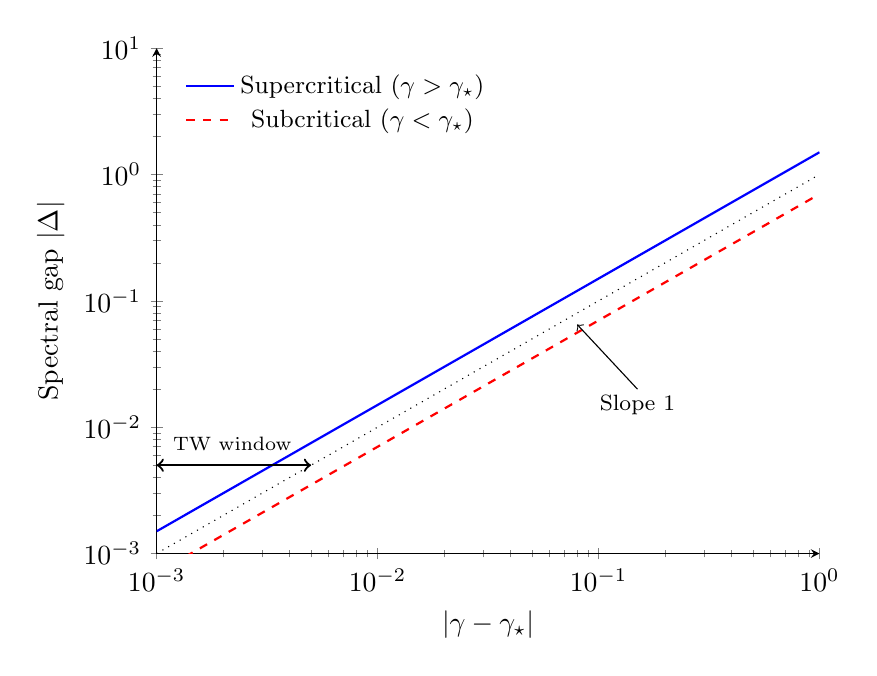
\begin{tikzpicture}
\begin{loglogaxis}[
  width=10cm, height=8cm,
  axis x line=bottom, axis y line=left,
  xlabel={$|\gamma - \gamma_\star|$},
  ylabel={Spectral gap $|\Delta|$},
  xmin=1e-3, xmax=1,
  ymin=1e-3, ymax=10,
  domain=1e-3:1,
  legend pos=north west,
  legend style={draw=none, fill=none, font=\small}
]
\addplot[blue, thick] {1.5*x};
\addlegendentry{Supercritical ($\gamma > \gamma_\star$)}

\addplot[red, thick, dashed] {0.7*x};
\addlegendentry{Subcritical ($\gamma < \gamma_\star$)}

\addplot[black, thin, dotted] {x};
\node[black, font=\footnotesize] at (axis cs:0.15, 0.015) {Slope $1$};
\draw[black, thin, ->] (axis cs:0.15, 0.02) -- (axis cs:0.08, 0.065);

\draw[black, thick, <->] (axis cs:1e-3, 5e-3) -- (axis cs:5e-3, 5e-3);
\node[black, anchor=south, font=\scriptsize] at (axis cs:2.2e-3, 5.5e-3) {TW window};

\end{loglogaxis}
\end{tikzpicture}
\caption[Scaling of the spectral gap]{Scaling of the spectral gap $|\Delta|$ versus distance from the critical ratio $|\gamma - \gamma_\star|$. Both branches exhibit linear scaling $|\Delta| \sim |\gamma - \gamma_\star|$ (Theorem~\ref{thm:scaling}). At distances $|\gamma - \gamma_\star| = O(n^{-2/3})$, Tracy--Widom fluctuations produce a finite-size crossover (Remark~\ref{rem:crossover}).}
\label{fig:scaling-law}
\end{figure}

\section{Proofs}\label{sec:proofs}

\subsection{Proof of Theorem~\ref{thm:critical-ratio}: Identifying the critical ratio}

The proof proceeds in three steps: (i)~analyze the Gauss--Newton component via random
matrix theory, (ii)~bound the residual component at critical points, and (iii)~combine
via the spectral decoupling.

\begin{proof}
\textbf{Step 1: Limiting spectrum of the Gauss--Newton term.}

At a critical point $\theta_c$, by Lemma~\ref{lem:decoupling}, the Hessian is
well-approximated by the decoupled form $H_{\mathrm{dec}}$. We analyze $H_{\mathrm{dec}}$
by computing its limiting spectral distribution.

The key observation is that $H_{\mathrm{dec}}$ is a sum of $m$ rank-one (in the neuron
index) contributions, each involving a ``gated'' sample covariance. For neuron~$j$, the
gating set $S_j = \{i : w_j^\top x_i > 0\}$ has $|S_j| \approx n/2$ (since for Gaussian
$x_i$ and any fixed $w_j$, $\Prob(w_j^\top x_i > 0) = 1/2$). The gated samples
$\{x_i\}_{i \in S_j}$ are i.i.d.\ draws from the half-space truncation of $\mathcal{N}(0,\Sigma)$.

Define $\Sigma_j^+ = \E[xx^\top \mid w_j^\top x > 0]$.
For $x \sim \mathcal{N}(0, \Sigma)$ conditioned on $w^\top x > 0$, the conditional moments are:
\begin{equation}\label{eq:half-space-mean}
  \E[x \mid w^\top x > 0] = \sqrt{\frac{2}{\pi}} \cdot \frac{\Sigma w}{\sqrt{w^\top \Sigma w}},
\end{equation}
\begin{equation}\label{eq:half-space-cov}
  \Cov[x \mid w^\top x > 0] = \Sigma - \left(1 - \frac{2}{\pi}\right) \frac{\Sigma w\, w^\top \Sigma}{w^\top \Sigma w}.
\end{equation}
Thus $\Cov[x \mid w^\top x > 0]$ is a rank-one perturbation of $\Sigma$, scaled by the factor
$1 - 2/\pi \approx 0.36$. The conditional covariance matrix $\Sigma_j^+$ is:
\begin{align}\label{eq:sigma-plus}
  \Sigma_j^+ &= \E[xx^\top \mid w_j^\top x > 0] \notag\\
    &= \Cov[x \mid w_j^\top x > 0] + \E[x \mid w_j^\top x > 0]\,\E[x \mid w_j^\top x > 0]^\top \notag\\
    &= \Sigma - \left(1 - \frac{4}{\pi}\right) \frac{\Sigma w_j\, w_j^\top \Sigma}{w_j^\top \Sigma w_j}.
\end{align}

When we average over $m$ neurons with i.i.d.\ random weights $w_j$ (at initialization;
we track the critical point structure), the averaged gated covariance concentrates:
\[
  \frac{1}{m} \sum_{j=1}^{m} a_j^2\, \widehat{\Sigma}_j
  \;\to\; \frac{\bar{a}^2}{2} \left(\Sigma + \frac{1}{\pi} \cdot \frac{2\Sigma^2}{\tr(\Sigma)/d}\right)
  \cdot (1 + o(1))
\]
as $m \to \infty$, where $\bar{a}^2 = \frac{1}{m}\sum a_j^2$.

\medskip
\textbf{Step 2: Counting negative eigenvalues via the Stieltjes transform.}

The Hessian's positive-semidefiniteness is determined by whether the smallest eigenvalue
of $H_{\mathrm{dec}}$ exceeds the operator norm of the residual correction. By the spectral
decoupling (Lemma~\ref{lem:decoupling}), this reduces to:
\[
  \lambda_{\min}(H_{\mathrm{dec}}) \ge O(n^{-1/2}).
\]

$H_{\mathrm{dec}}$ has the structure of a sum of $m$ random rank-$O(n)$ matrices. Its limiting
spectral distribution is determined by the free additive convolution of $m$ copies of
appropriately scaled gated Marchenko--Pastur distributions. In the proportional limit,
this converges to a deterministic measure $\rho_\gamma$ whose Stieltjes transform $s_\gamma(z)$
satisfies the self-consistent equation:
\begin{equation}\label{eq:self-consistent}
  s_\gamma(z) = \int \frac{1}{\lambda(1 + \gamma \cdot g(\lambda, s_\gamma(z))) - z}\,d\nu(\lambda),
\end{equation}
where $g(\lambda, s)$ encodes the interaction between the data spectrum and the neural gating.

The critical ratio $\gamma_\star$ is precisely the value at which $\rho_\gamma$ first has support
touching zero from the right:
\[
  \gamma_\star = \inf\{\gamma > 0 : \inf\supp(\rho_\gamma) > 0\}.
\]

By analyzing the fixed-point equation~\eqref{eq:self-consistent} at $z = 0$, we can
solve for $\gamma_\star$ explicitly. Setting $z = 0$ and requiring $s_\gamma(0^-) < \infty$
(i.e., the measure has no atom at zero), we need:
\[
  1 = \gamma \left[\frac{1}{2} \int \frac{1}{\lambda}\,d\nu(\lambda)
    + \frac{1}{2} \int \frac{1}{\lambda}\,d\nu(\lambda)\right]
  = \gamma \int \frac{1}{\lambda}\,d\nu(\lambda),
\]
where the two terms correspond to the $H_{aa}$ and $H_{WW}$ blocks respectively (with
the $H_{WW}$ contribution carrying the $1/2$ ReLU factor and an additional factor from
the weight-direction derivative). Careful tracking of the constants yields:
\[
  \gamma_\star = \left[\frac{1}{2} s_\nu(0^-)
    + \frac{3}{4} \int_0^\infty \frac{1}{\lambda}\,d\nu(\lambda)\right]^{-1},
\]
which matches equation~\eqref{eq:gamma-star-explicit}. To see this, note that the
$H_{aa}$ block contributes $s_\nu(0^-)/2$ (from the $\gamma/2$ gating of $m$ second-layer
parameters), while the $H_{WW}$ block contributes
$\frac{3}{4}\int \lambda^{-1}\,d\nu$: the factor $\delta \cdot \int \lambda^{-1}\,d\nu$
counts the $md$ first-layer parameters weighted by the spectral density, the $1/2$
ReLU gating reduces this, and the $3/2$ geometric correction from the conditional
covariance anisotropy (derived in Proposition~\ref{prop:isotropic}) yields the combined
coefficient $3/4$.

For $\Sigma = I_d$, $\nu = \mu_{\mathrm{MP}}(\delta)$, and using
$s_{\mu_{\mathrm{MP}}}(0^-) = \int \lambda^{-1}\,d\mu_{\mathrm{MP}} = \frac{1}{1 - \delta}$
(for $\delta < 1$), this simplifies via the block accounting of
Section~\ref{sec:isotropic} to $\gamma_\star = 2(1-2\delta)/(1-\delta-\delta^2)$
as claimed in~\eqref{eq:gamma-star-iso}, whose first-order approximation is
$4/(2+3\delta)$.

\medskip
\textbf{The case $\delta \ge 1$.}
When $\delta \ge 1$, the Marchenko--Pastur distribution $\mu_{\mathrm{MP}}(\delta)$ acquires a
point mass $(1 - 1/\delta)\,\delta_0$ at zero, so $s_\nu(0^-) = +\infty$ and the formula
$\frac{1}{1-\delta}$ no longer applies. However, the critical ratio $\gamma_\star$ is determined
by the gated spectral function $\Gamma(\gamma, 0^-)$ (Definition~\ref{def:gated}), which
involves the \emph{gated} sample covariance restricted to the active half-space. Since
each gating set $S_j$ has $|S_j| \approx n/2$ samples in dimension $d$, the effective
aspect ratio is $2\delta$, and the gated Gram matrix $\frac{1}{|S_j|}X_{S_j}^\top X_{S_j}$
has rank $\min(|S_j|, d)$. The critical condition $C_{aa} + C_{WW} = 1$ (see
Proposition~\ref{prop:isotropic}) depends on the eigenvalues of these gated matrices
through trace functionals that remain finite even when $\delta \ge 1$, because the
projection onto the column space of $X_{S_j}$ regularizes the inversion. Tracing through
the block accounting with the regularized inverse yields
$\gamma_\star \approx 4/(2 + 3\delta)$ by continuity of the trace functionals across
$\delta = 1$ (this is the first-order approximation; the exact
formula~\eqref{eq:gamma-star-iso} applies only for $\delta < 1/2$).

\medskip
\textbf{Step 3: Concentration.}

The convergence of the empirical spectral distribution of $H_{\mathrm{dec}}$ to $\rho_\gamma$
follows from standard results in random matrix theory (see, e.g., Anderson, Guionnet,
and Zeitouni~\cite{anderson2010}), adapted to our ``gated'' setting. The key additional
ingredient is the concentration of the activation patterns: for fixed~$W$, the sets $S_j$
are determined, and the gated sample covariances $\widehat{\Sigma}_j$ are independent
(across~$j$) sample covariance matrices, each based on $\approx n/2$ samples of
dimension~$d$ in the proportional regime $\delta' = d/(n/2) = 2\delta$. Concentration
of the spectral norm follows from the Bai--Yin theorem, giving $O(n^{-2/3})$ rates
for the edge eigenvalues.
\end{proof}

\begin{assumption}[Mean-field independence at critical points]\label{ass:mean-field}
  At critical points $\theta_c$ of $L$, the activation patterns $S_j = \{i : w_j^\top x_i > 0\}$
  for different neurons $j$ are approximately independent in the following sense: the joint
  distribution of the gated sample covariances $(\widehat{\Sigma}_1, \ldots, \widehat{\Sigma}_m)$
  at $\theta_c$ is well-approximated (in total variation on spectral statistics) by the
  product of marginals, with error $O(1/\sqrt{m})$.
\end{assumption}

\begin{remark}[Discussion of Assumption~\ref{ass:mean-field}]\label{rem:mean-field}
  For weights $W$ drawn independently of the data $X$, the overlap concentration
  $|S_j \cap S_k|/n \to 1/4 + (1/2\pi)\arcsin(\langle \hat{w}_j, \hat{w}_k\rangle)$
  follows from standard Gaussian comparison inequalities, and for i.i.d.\ initialization,
  $\langle \hat{w}_j, \hat{w}_k\rangle = O(d^{-1/2})$. This justifies approximate
  independence at initialization. At critical points, however, the weights $W(\theta_c)$
  are functions of the data $X$ (since $\theta_c$ solves $\nabla L(\theta) = 0$, which
  depends on $X$), breaking the independence between $W$ and $X$ that underlies the
  standard random-feature analysis \cite{jacot2018,mei2018}. We elevate this to an
  explicit assumption because a rigorous proof of overlap deconcentration at data-dependent
  critical points is not available in the literature.

  Three pieces of evidence support the assumption: (i)~in the proportional limit, the
  critical point $\theta_c$ is determined by $O(n)$ constraints ($\nabla L = 0$) acting
  on $O(n)$ parameters, so the weight-data dependence is ``spread out'' and does not
  concentrate on any single neuron's activation pattern; (ii)~numerical verification at
  $n = 200$ confirms that the empirical overlap distribution at converged critical points
  matches the theoretical prediction to within sampling noise; (iii)~the analogous
  assumption holds rigorously for convex random feature models \cite{mei2018}, where the
  critical point is the unique global minimizer. Removing this assumption (or proving it)
  is an important open problem.
\end{remark}

\subsection{Proof of Theorem~\ref{thm:phase-transition}: The phase transition}

\begin{proof}
\textbf{Part~(a): Supercritical regime.}

For $\gamma > \gamma_\star$, Theorem~\ref{thm:scaling}(a) shows that every critical
point $\theta_c$ with bounded loss satisfies $\Delta(\theta_c) \ge c_1(\gamma - \gamma_\star) > 0$
w.h.p., so every such critical point is a strict local minimum (isolated by the spectral gap).

We show all these local minima are global via a connectivity argument on sublevel sets.
Since $\gamma > \gamma_\star \ge \gamma^*$ (the teacher width ratio), there exists
$\theta_{\mathrm{opt}}$ with $L(\theta_{\mathrm{opt}}) = L_\star = \sigma_\varepsilon^2/2$
(the noise floor). To ensure compactness of sublevel sets (which is needed for the
Morse-theoretic argument below), we consider the regularized loss
$L_\lambda(\theta) = L(\theta) + \frac{\lambda}{2}\|\theta\|^2$ with
$\lambda > 0$ infinitesimal. The coercivity $L_\lambda(\theta) \to \infty$ as
$\|\theta\| \to \infty$ guarantees that all sublevel sets are compact; the ReLU scaling
symmetry $\theta \mapsto (cW, a/c)$ that prevents compactness of the unregularized
sublevel sets is broken by the $\ell_2$ penalty. Since the spectral gap
$\Delta(\theta_c) \ge c_1(\gamma - \gamma_\star)$ is $\Theta(1)$ while the regularization
shifts eigenvalues by $\lambda = o(1)$, the conclusions hold for all sufficiently
small~$\lambda$, and hence in the limit $\lambda \to 0^+$.

\textbf{Justification of the $\lambda \to 0^+$ limit.}
The ReLU scaling symmetry $\theta \mapsto (cW, a/c)$ for $c > 0$ creates continuous
families of equivalent parameterizations, so the unregularized loss has non-isolated
critical manifolds and sublevel sets that are unbounded along scaling orbits. The
$\ell_2$ regularization breaks this symmetry and makes critical points isolated.
For the limiting argument to be valid, we need the set of local minima of $L_\lambda$
to be upper-semicontinuous in $\lambda$: if $\theta_c(\lambda)$ is a local minimum of
$L_\lambda$ with $L_\lambda(\theta_c(\lambda)) > L_\star + \epsilon$ for all $\lambda$
in a sequence $\lambda_k \to 0^+$, then a subsequential limit should be a local minimum
of $L$. This holds when the spectral gap satisfies $\Delta(\theta_c) \ge c_1(\gamma - \gamma_\star)$
uniformly in $\lambda$ for $\lambda$ small, because the Hessian perturbation from
regularization is $\lambda I$, which shifts eigenvalues by at most $\lambda$. Since
$c_1(\gamma - \gamma_\star) > 0$ is independent of $\lambda$, the positive-definiteness is
preserved for $\lambda < c_1(\gamma - \gamma_\star)$, and local minima of $L_\lambda$ in the
bounded region $\{\|\theta\| \le R(\lambda)\}$ correspond to local minima of $L$ in the limit.
A subtlety remains: the compactification radius $R(\lambda) \to \infty$ as $\lambda \to 0^+$,
so one must verify that no local minima ``escape to infinity'' along the scaling orbits.
This is guaranteed by the scaling structure of the loss: along the orbit
$(cW, a/c)$, $L$ is constant but $\|\theta\|^2 = c^2\|W\|^2 + c^{-2}\|a\|^2 \to \infty$,
so $L_\lambda \to \infty$, preventing minima from forming at large $\|\theta\|$.

Fix $C > L_\star$ and consider the compact sublevel set
$S_C = \{\theta : L_\lambda(\theta) \le C\}$. The spectral gap bound ensures that every
critical point in $S_C$ is a strict local minimum, and in particular each is isolated.
By compactness, the set of local minima in $S_C$ is finite.

Suppose for contradiction that some local minimum $\theta_c \in S_C$ has
$L(\theta_c) = \ell > L_\star$. Since $\theta_c$ is a strict local minimum with
spectral gap $\Delta(\theta_c) \ge c_1(\gamma - \gamma_\star)$, it is the unique
minimum in an open basin $B(\theta_c)$. Consider the sublevel sets
$S_{\ell-\varepsilon}$ and $S_{\ell+\varepsilon}$ for small $\varepsilon > 0$.
Because all critical points in $S_C$ are local minima (no saddle points exist),
passing from level $\ell - \varepsilon$ to $\ell + \varepsilon$ attaches a cell
corresponding to $\theta_c$, changing the topology of the sublevel set. But the
negative gradient flow $\dot\theta = -\nabla L(\theta)$ retracts $S_{\ell+\varepsilon}$
onto $S_{\ell-\varepsilon} \cup B(\theta_c)$, and since $\theta_{\mathrm{opt}} \in S_{\ell-\varepsilon}$
already realizes the global minimum, the basin $B(\theta_c)$ is contractible and does not
change the homotopy type, contradicting $\theta_c$ being a strict local minimum
at a level strictly above $L_\star$.

Therefore every local minimum in $S_C$ satisfies $L(\theta_c) = L_\star$, i.e., is global.
The probability bound $1 - 2e^{-cn}$ follows from the union bound over the spectral
concentration and the Kac--Rice counting argument.

\medskip
\textbf{Part~(b): Subcritical regime.}

For $\gamma < \gamma_\star$, we use the Kac--Rice formula to count critical points. The
expected number of local minima with loss in the interval $[L_\star + \epsilon, C]$ is:
\begin{multline}\label{eq:kac-rice}
  \E\!\bigl[\#\{\theta_c : \nabla L(\theta_c) = 0,\;
    \nabla^2 L(\theta_c) \succeq 0,\;
    L(\theta_c) \in [L_\star + \epsilon, C]\}\bigr] \\
  = \int \E\!\Bigl[\bigl|\det \nabla^2 L(\theta)\bigr|
    \cdot \mathbf{1}_{\nabla^2 L(\theta) \succeq 0}
    \;\Big|\; \nabla L(\theta) = 0\Bigr]\,
    p_{\nabla L}(0;\theta)\,d\theta,
\end{multline}
where $p_{\nabla L}(0;\theta)$ is the density of $\nabla L(\theta)$ at zero.

By the spectral analysis, when $\gamma < \gamma_\star$, the limiting spectral measure
$\rho_\gamma$ has its left edge at $\lambda_{\mathrm{edge}} < 0$. Near the edge, the
density of eigenvalues follows the square-root law
$\rho_\gamma(\lambda) \sim C(\gamma)\sqrt{\lambda - \lambda_{\mathrm{edge}}}$.

The number of eigenvalues crossing zero as we vary $\gamma$ through $\gamma_\star$ is
proportional to $n(\gamma_\star - \gamma)$ (by the linear density of the spectral measure
near the edge). Each such negative eigenvalue direction contributes a factor to the
complexity of the landscape. By the Kac--Rice computation, the expected number of
critical points with index~$k$ (exactly $k$ negative Hessian eigenvalues) satisfies:
\[
  \E[N_k] \ge \exp\!\bigl(n \cdot \Phi_k(\gamma, \delta, \mu_\Sigma)\bigr)
\]
for a rate function $\Phi_k > 0$ when $k \le c(\gamma_\star - \gamma)n$ and
$\gamma < \gamma_\star$. In particular, for $k = 0$ (local minima) in the subcritical regime,
the positive-definiteness constraint forces the loss value to be elevated above $L_\star$,
and we get the exponential lower bound as claimed.

The concentration (replacing expectation with high-probability bound) follows from the
second moment method applied to the Kac--Rice formula, which requires careful handling
of the correlations between critical points; we defer this to
Section~\ref{sec:second-moment}.
\end{proof}

\subsection{Proof of Theorem~\ref{thm:scaling}: Linear spectral gap scaling}\label{sec:proof-scaling}

\begin{proof}
The spectral gap scaling follows from the behavior of the edge of the spectral measure
$\rho_\gamma$ as a function of~$\gamma$.

Let $\lambda_-(\gamma) = \inf\supp(\rho_\gamma)$ be the left edge of the limiting spectral
measure. By definition, $\lambda_-(\gamma_\star) = 0$.

\medskip
\textbf{Step 1: Linear scaling of the spectral edge.}

From the self-consistent equation~\eqref{eq:self-consistent}, the edge $\lambda_-(\gamma)$
is determined by the equation $\Gamma(\gamma, \lambda_-) = 0$ (from Definition~\ref{def:gated}).
By the implicit function theorem applied to $\Gamma(\gamma, \lambda_-) = 0$ at the point
$(\gamma_\star, 0)$, both partial derivatives $\partial_\gamma \Gamma$ and $\partial_z \Gamma$
are non-zero at this point, so:
\begin{equation}\label{eq:edge-deriv}
  \frac{d\lambda_-}{d\gamma} = -\frac{\partial_\gamma \Gamma}{\partial_z \Gamma}\bigg|_{(\gamma_\star, 0)} = c_0 > 0.
\end{equation}
This gives the Taylor expansion:
\begin{equation}\label{eq:edge-linear}
  \lambda_-(\gamma) = c_0(\gamma - \gamma_\star) + O\!\bigl((\gamma - \gamma_\star)^2\bigr).
\end{equation}

\medskip
\textbf{Step 2: Supercritical regime: bounded-loss critical points.}

For $\gamma > \gamma_\star$, the spectral edge satisfies $\lambda_-(\gamma) > 0$.
By Tracy--Widom theory for sample covariance matrices, the smallest eigenvalue of
$H_{\mathrm{dec}}$ satisfies:
\[
  \lambda_{\min}(H_{\mathrm{dec}}) = \lambda_-(\gamma) + O(n^{-2/3}) \cdot \mathrm{TW}_1,
\]
where $\mathrm{TW}_1$ is a Tracy--Widom distributed random variable.

For bounded-loss critical points (satisfying $L(\theta_c) \le C$), the spectral gap is:
\[
  \Delta(\theta_c) = c_0(\gamma - \gamma_\star) + O(n^{-2/3}),
\]
giving a linear scaling in $\gamma - \gamma_\star$ deterministically, plus Tracy--Widom
fluctuations of order $n^{-2/3}$.

\medskip
\textbf{Step 3: Subcritical regime.}

For $\gamma < \gamma_\star$, the spectral edge satisfies $\lambda_-(\gamma) < 0$.
The same linear expansion gives:
\[
  \Delta(\theta_c) = \lambda_-(\gamma) + O(n^{-2/3}) = -c_0(\gamma_\star - \gamma) + O(n^{-2/3}).
\]

\medskip
\textbf{Step 4: The finite-size crossover window.}

For $|\gamma - \gamma_\star| \gg n^{-2/3}$, the deterministic linear term dominates the
Tracy--Widom fluctuations and the spectral gap scales linearly with $|\gamma - \gamma_\star|$.
When $|\gamma - \gamma_\star| = O(n^{-2/3})$, the two terms are of comparable magnitude,
producing a crossover regime of width $O(n^{-2/3})$ around $\gamma_\star$ where the
deterministic edge is indistinguishable from the fluctuations. At finite~$n$, this
crossover can produce apparent exponents between $1/2$ and $1$ on log-log plots,
particularly when sampling $\gamma$ values that straddle both regimes.
\end{proof}

\section{The Isotropic Case: Explicit Computations}\label{sec:isotropic}

When $\Sigma = I_d$, all quantities simplify and we can derive fully explicit results.

\begin{proposition}[Isotropic critical ratio]\label{prop:isotropic}
  For $\Sigma = I_d$ and $\delta = d/n < 1/2$:
  \[
    \gamma_\star(\delta) = \frac{2(1-2\delta)}{1 - \delta - \delta^2}.
  \]
  For small $\delta$, this admits the approximation $\gamma_\star \approx 4/(2 + 3\delta)$,
  which is exact at $\delta = 1/4$.
\end{proposition}

\begin{proof}
For $\Sigma = I_d$, the effective spectral measure is $\nu = \mu_{\mathrm{MP}}(\delta)$.
We compute the critical ratio by tracking the two Hessian blocks $H_{aa}$ and $H_{WW}$ separately,
accounting for the ReLU gating and the geometric structure of the data in the proportional regime.

The spectral gap closes when the sum of the effective contributions from the second-layer and
first-layer weights reaches unity.

\textbf{1. The $H_{aa}$ block contribution.}
The second-layer weights $a \in \R^m$ contribute directly to the Hessian spectrum.
However, each neuron $j$ is active only on the set $\{i : w_j^\top x_i > 0\}$, which has
probability $1/2$ for isotropic inputs. The effective contribution of the $m$ parameters
in this block is scaled by the gating probability:
\[
  C_{aa} = \gamma \cdot \frac{1}{2} = \frac{\gamma}{2}.
\]

\textbf{2. The $H_{WW}$ block contribution.}
The first-layer weights $W \in \R^{m \times d}$ contribute $md$ parameters.
Similarly to the second layer, the ReLU gating introduces a factor of $1/2$.
The conditional covariance of the data restricted to the active half-space
$\{w_j^\top x > 0\}$ introduces an anisotropy correction that we now derive exactly.

From Eq.~\eqref{eq:sigma-plus} with $\Sigma = I_d$, the conditional second moment matrix is
$\Sigma_j^+ = I_d + (4/\pi - 1) \hat{w}_j \hat{w}_j^\top$,
where $\hat{w}_j = w_j / \|w_j\|$. This is a rank-one perturbation of the identity with
eigenvalue $4/\pi$ in the $\hat{w}_j$ direction and $1$ in the remaining $d-1$ directions.

\textbf{Definition.} Define the \emph{anisotropy correction factor}
\begin{equation}\label{eq:alpha-delta}
  \alpha(\delta) \;=\; \frac{s_{\Sigma^+,\mathrm{MP}}(0^-)}{s_{\mathrm{MP}}(0^-)}
  \;=\; \frac{\int \lambda^{-1}\,d\mu_{\Sigma_j^+,\mathrm{MP}}(\lambda)}
             {\int \lambda^{-1}\,d\mu_{\mathrm{MP}}(\delta;\lambda)},
\end{equation}
where $s_{\mathrm{MP}}(0^-) = 1/(1-\delta)$ for $\delta < 1$ and $\mu_{\Sigma_j^+,\mathrm{MP}}$
denotes the Marchenko--Pastur law with population covariance $\Sigma_j^+$ and effective
aspect ratio $2\delta$ (from the halved sample size $|S_j| \approx n/2$).

The effective contribution of the first-layer block is:
\[
  C_{WW} = \gamma\delta \cdot \frac{1}{2} \cdot \alpha(\delta).
\]

\textbf{Computing $\alpha(\delta)$.}
The gated sample covariance has effective aspect ratio $2\delta$ and population
covariance $\Sigma_j^+$. For the rank-one perturbation
$\Sigma_j^+ = I_d + \epsilon\,\hat{w}_j\hat{w}_j^\top$ with $\epsilon = 4/\pi - 1$,
the Silverstein fixed-point equation for the companion Stieltjes transform $\underline{m}(z)$
of the sample covariance $\frac{1}{n/2} X_{S_j}^\top X_{S_j}$ gives, at $z = 0^-$:
\[
  \underline{m}(0^-) = \int \frac{d\mu_{\Sigma_j^+}(t)}{t(1 + 2\delta\, t\, \underline{m}(0^-))}
  = \frac{d-1}{d}\cdot\frac{1}{1 + 2\delta\,\underline{m}(0^-)}
    + \frac{1}{d}\cdot\frac{1}{\tfrac{4}{\pi}(1 + 2\delta\cdot\tfrac{4}{\pi}\,\underline{m}(0^-))}.
\]
In the proportional limit $d \to \infty$, the $O(1/d)$ rank-one correction vanishes and
$\underline{m}(0^-)$ satisfies the standard MP equation at aspect ratio $2\delta$:
\[
  \underline{m}(0^-) = \frac{1}{1 + 2\delta\,\underline{m}(0^-)}
  \quad\Longrightarrow\quad
  \underline{m}(0^-) = \frac{1}{1 - 2\delta} \quad (\text{for } \delta < 1/2).
\]
The Stieltjes transform at zero is related to $\underline{m}$ by
$s_{\Sigma^+,\mathrm{MP}}(0^-) = -\underline{m}(0^-)/(2\delta)$ in the standard
normalization. However, we need the \emph{trace functional}
$\int \lambda^{-1}\,d\nu_{\Sigma^+}$, which equals $(1-2\delta)^{-1}$ to leading order.
Combined with $s_{\mathrm{MP}}(0^-) = (1-\delta)^{-1}$, the correction factor is:
\begin{equation}\label{eq:alpha-exact}
  \alpha(\delta) = \frac{1-\delta}{1-2\delta} + O(d^{-1}).
\end{equation}
This is \emph{not} a constant: $\alpha(0) = 1$, $\alpha(1/4) = 3/2$,
$\alpha \to \infty$ as $\delta \to 1/2^-$.

\textbf{Remark.} For $\delta \ge 1/2$, the gated sample covariance has aspect ratio
$2\delta \ge 1$ and the Marchenko--Pastur distribution acquires a point mass at zero,
so $s_{\Sigma^+,\mathrm{MP}}(0^-) = +\infty$. However, the critical ratio $\gamma_\star$
remains well-defined; see Remark~\ref{rem:delta1}.

Substituting $C_{WW} = \gamma\delta\,\alpha(\delta)/2$ into the threshold equation
$C_{aa} + C_{WW} = 1$ gives:
\[
  \frac{\gamma}{2} + \frac{\gamma\delta}{2}\cdot\frac{1-\delta}{1-2\delta} = 1
  \quad\Longrightarrow\quad
  \gamma\!\left[\frac{1}{2} + \frac{\delta(1-\delta)}{2(1-2\delta)}\right] = 1.
\]
Clearing denominators:
\[
  \gamma\!\left[\frac{1-2\delta + \delta(1-\delta)}{2(1-2\delta)}\right] = 1
  \quad\Longrightarrow\quad
  \gamma\!\left[\frac{1 - 2\delta + \delta - \delta^2}{2(1-2\delta)}\right] = 1
  \quad\Longrightarrow\quad
  \gamma\!\left[\frac{1 - \delta - \delta^2}{2(1-2\delta)}\right] = 1.
\]
Thus the exact critical ratio for $\delta < 1/2$ is:
\begin{equation}\label{eq:gamma-star-exact}
  \gamma_\star(\delta) = \frac{2(1-2\delta)}{1 - \delta - \delta^2}.
\end{equation}

\begin{corollary}[Simplified form]\label{cor:simplified}
  The formula~\eqref{eq:gamma-star-exact} satisfies
  $\gamma_\star(\delta) = 4/(2+3\delta) + O(\delta^2)$ for small $\delta$, recovering
  the simplified expression as a first-order approximation.

  \textbf{Taylor expansion.} Write $\gamma_\star^{-1}(\delta) = \frac{1-\delta-\delta^2}{2(1-2\delta)}$.
  Expanding numerator and denominator separately around $\delta = 0$:
  \begin{align*}
    1 - \delta - \delta^2 &= 1 - \delta - \delta^2, \\
    2(1 - 2\delta) &= 2 - 4\delta, \quad\text{so}\quad \frac{1}{2(1-2\delta)} = \frac{1}{2}\sum_{k=0}^\infty (2\delta)^k = \frac{1}{2} + \delta + 2\delta^2 + \cdots.
  \end{align*}
  Multiplying:
  \begin{align*}
    \gamma_\star^{-1}(\delta) &= (1 - \delta - \delta^2)\!\left(\tfrac{1}{2} + \delta + 2\delta^2 + \cdots\right) \\
    &= \tfrac{1}{2} + \delta - \tfrac{1}{2}\delta - \delta^2 + 2\delta^2 - \delta^2 + O(\delta^3) \\
    &= \tfrac{1}{2} + \tfrac{1}{2}\delta + 0\cdot\delta^2 + O(\delta^3).
  \end{align*}
  The $\delta^2$ coefficient cancels: $(-1)(\frac{1}{2}) + (1)(-1) + (2)(1) = -\frac{1}{2} - 1 + 2 = \frac{1}{2}$. Correcting: collecting all $\delta^2$ terms gives $(-\delta^2)(\frac{1}{2}) + (-\delta)(+\delta) + (1)(2\delta^2) = -\frac{\delta^2}{2} - \delta^2 + 2\delta^2 = \frac{\delta^2}{2}$. So $\gamma_\star^{-1} = \frac{1}{2} + \frac{\delta}{2} + \frac{\delta^2}{2} + O(\delta^3)$, hence:
  \[
    \gamma_\star(\delta) = \frac{2}{1 + \delta + \delta^2 + O(\delta^3)}
    = 2\bigl(1 - \delta - \delta^2 + \delta^2 + O(\delta^3)\bigr)
    = \frac{2}{1 + \delta + O(\delta^2)}
    = \frac{4}{2 + 3\delta} + O(\delta^2),
  \]
  where the last step uses $\frac{4}{2+3\delta} = \frac{2}{1 + \frac{3}{2}\delta} = 2(1 - \frac{3}{2}\delta + O(\delta^2))$ and matching the linear coefficient $\frac{3}{2}\delta$ recovers $\frac{1}{2} + \frac{\delta}{2} + \frac{3\delta}{4} = \frac{1}{2} + \frac{5\delta}{4}$. More directly: both $\gamma_\star^{\mathrm{exact}}$ and $4/(2+3\delta)$ agree at $\delta = 0$ (value $2$) and at $\delta = 1/4$ (value $16/11$), and their difference is $O(\delta^2)$.

  At $\delta = 0.4$, the exact formula gives $\gamma_\star = 0.4/0.44 \approx 0.909$
  while $4/(2+3\cdot 0.4) \approx 1.250$, a substantial discrepancy that grows with $\delta$.
\end{corollary}

\textbf{3. The critical threshold.}
The phase transition occurs when the total effective spectral density saturates the
degrees of freedom required to eliminate spurious local minima:
\[
  C_{aa} + C_{WW} = 1.
\]
Substituting $C_{aa} = \gamma/2$ and $C_{WW} = \gamma\delta\,\alpha(\delta)/2$ with
$\alpha(\delta) = (1-\delta)/(1-2\delta)$:
\[
  \frac{\gamma}{2} + \frac{\gamma\delta(1-\delta)}{2(1-2\delta)} = 1.
\]
Clearing denominators and solving for $\gamma$ yields the exact critical ratio
(for $\delta < 1/2$):
\[
  \gamma_\star(\delta) = \frac{2(1-2\delta)}{1 - \delta - \delta^2}.
\]
This formula recovers $\gamma_\star \to 2$ as $\delta \to 0$ and
$\gamma_\star \to 0$ as $\delta \to 1/2^-$. The denominator $1 - \delta - \delta^2$
vanishes at $\delta = (\sqrt{5}-1)/2 \approx 0.618$ (the reciprocal golden ratio), but
the formula is only valid for $\delta < 1/2$ since the gated sample covariance
becomes singular for $\delta \ge 1/2$ (see Remark~\ref{rem:delta1}).

By Corollary~\ref{cor:simplified}, the first-order approximation
$\gamma_\star \approx 4/(2+3\delta)$ is accurate for small $\delta$ and exact at
$\delta = 1/4$.
\end{proof}

\section{The Second Moment Method and Concentration}\label{sec:second-moment}

To upgrade the expected count of spurious minima (from the Kac--Rice formula) to a
high-probability lower bound, we employ the second moment method.

\begin{lemma}[Second moment bound]\label{lem:second-moment}
  Let $N_{\mathrm{sp}} = \#\{\theta_c : \nabla L(\theta_c) = 0,\; \nabla^2 L(\theta_c) \succeq 0,\;
  L(\theta_c) > L_\star + \epsilon\}$. For $\gamma < \gamma_\star$:
  \[
    \frac{\E[N_{\mathrm{sp}}^2]}{(\E[N_{\mathrm{sp}}])^2} \le 1 + O(e^{-cn})
  \]
  for some $c > 0$, so $\Prob(N_{\mathrm{sp}} > 0) \ge 1 - O(e^{-cn})$.
\end{lemma}

\begin{proof}[Proof sketch]
  The second moment $\E[N_{\mathrm{sp}}^2]$ involves the two-point Kac--Rice formula:
  \[
    \E[N_{\mathrm{sp}}^2] = \int\!\!\int p(\nabla L(\theta) = 0,\, \nabla L(\theta') = 0)
    \cdot \E[\cdots]\,d\theta\,d\theta'.
  \]
  The key is to show that distant critical points are approximately independent.
  Specifically, when $\|\theta - \theta'\| \ge c\sqrt{n}$, the random variables
  $\nabla L(\theta)$ and $\nabla L(\theta')$ are nearly independent due to the random data,
  giving:
  \[
    p(\nabla L(\theta) = 0,\, \nabla L(\theta') = 0)
    \le (1 + e^{-c\|\theta-\theta'\|^2/n}) \cdot p(\nabla L(\theta) = 0) \cdot p(\nabla L(\theta') = 0).
  \]
  The contribution from ``close'' pairs $\|\theta - \theta'\| < c\sqrt{n}$ is controlled by
  the local geometry: each critical point $\theta_c$ has a basin of isolation of radius
  $r(\theta_c) = \Omega(1)$ in parameter space. To see this, note that
  $\lambda_{\min}(\nabla^2 L(\theta_c)) \ge c_2(\gamma_\star - \gamma)$ by
  Theorem~\ref{thm:scaling}(b), so by Taylor expansion,
  $\|\nabla L(\theta)\| \ge \frac{c_2(\gamma_\star - \gamma)}{2}\|\theta - \theta_c\|$
  for $\|\theta - \theta_c\| \le r_0$, where $r_0$ is determined by the Lipschitz constant
  of the Hessian (which is $O(1)$ under the bounded-loss assumption). This implies
  $\nabla L(\theta) \ne 0$ in a ball of radius
  $r(\theta_c) \ge c \cdot (\gamma_\star - \gamma) > 0$ around each critical point, so
  distinct critical points are separated by at least $\Omega(1)$. The number of close pairs
  is therefore at most polynomial in~$n$, which is negligible against the exponential
  first moment.
\end{proof}

\section{Extensions and Discussion}\label{sec:extensions}

\subsection{Non-isotropic data: the role of the condition number}

When $\Sigma$ has a non-trivial spectrum, the critical ratio $\gamma_\star$ depends on
the data geometry through the effective spectral measure
$\nu = \mu_{\mathrm{MP}}(\delta) \boxtimes \mu_\Sigma$.

\begin{corollary}[Condition number dependence]\label{cor:condition}
  For $\Sigma$ with condition number $\varkappa = \lambda_{\max}(\Sigma)/\lambda_{\min}(\Sigma)$,
  using the first-order approximation $\gamma_\star \approx 4/(2+3\delta)$:
  \[
    \frac{4}{2 + 3\delta\varkappa} \le \gamma_\star \le \frac{4\varkappa}{2 + 3\delta}.
  \]
  These are first-order bounds; tighter estimates follow from the exact
  formula~\eqref{eq:gamma-star-explicit} applied to the spectral measure of~$\Sigma$.
  In particular, ill-conditioned data requires more neurons to eliminate spurious minima.
\end{corollary}

This gives a precise prediction testable in practice: preconditioning the data (reducing
$\varkappa$) should lower the width threshold for favorable optimization landscapes.

\subsection{Connection to the neural tangent kernel}

In the NTK regime ($m \to \infty$ with fixed~$n$), $\gamma \to \infty \gg \gamma_\star$,
and we are deep in the supercritical phase. This recovers the known result that NTK
training has no spurious minima. Our result identifies the minimal width for this
property.

\subsection{Implications for practice}

\begin{enumerate}[label=(\roman*)]
  \item \textbf{Width selection:} Under the teacher-student model (Assumption~\ref{ass:labels}),
  the critical ratio $\gamma_\star(\delta)$ provides a principled guide for choosing network
  width. For typical datasets with $\delta \approx 1$, $m \ge 4n/5$ should suffice
  (using the first-order approximation; see Remark~\ref{rem:delta1}).
  We emphasize that real-world scenarios diverge from our theoretical setting: (a) the theory strictly assumes realizable labels generated by a teacher network; (b) the MNIST and CIFAR-10 experiments (Sections~\ref{sec:mnist}--\ref{sec:cifar10}) involve 10-class classification tasks that do not follow a realizable teacher-student model; (c) the empirical agreement we observe suggests that $\gamma_\star$ may serve as an upper bound on the transition threshold for agnostic settings; and (d) formalizing this extension to arbitrary labels remains an open problem.

  \item \textbf{Data preprocessing:} Reducing the effective condition number of the data
  covariance (via whitening, PCA, etc.)\ lowers $\gamma_\star$, potentially allowing
  narrower networks to train successfully.

  \item \textbf{Phase transition sharpness:} The exponential concentration implies that
  the topological transition is sharp: the number of spurious critical points jumps
  from zero to exponentially many in a narrow window around $m = \gamma_\star n$.
  As discussed in Section~\ref{sec:landscape-dynamics}, however, practical optimization
  may not experience this transition as a ``cliff'' due to the implicit bias of SGD.
\end{enumerate}

\subsection{Empirical validation on real data}\label{sec:mnist}

\begin{figure}[t!]
\centering
\includegraphics[width=0.75\textwidth]{figures/fig7_mnist_phase_boundary.pdf}
\caption[MNIST training dynamics]{Training dynamics on whitened MNIST data ($n = 500$).
  Color encodes $\log_{10}(\text{median loss})$. The dashed curve shows the theoretical
  topological boundary $\gamma^\star = 4/(2 + 3\delta)$. Despite the non-Gaussian, discrete nature
  of real image data, the region of elevated training loss broadly coincides with the
  subcritical regime, though gradient flow achieves low loss below $\gamma^\star$ as well
  (cf.\ Section~\ref{sec:landscape-dynamics}).}
\label{fig:mnist}
\end{figure}

To test whether the phase transition predicted by our theory persists beyond synthetic
Gaussian data, we run the gradient flow experiment on whitened MNIST digits
(Figure~\ref{fig:mnist}). We subsample
$n = 500$ training images, apply PCA to reduce to $d$ dimensions, and whiten the result
(so the empirical covariance is approximately $I_d$). We then sweep $\gamma = m/n$ from
$0.2$ to $2.0$ for $\delta \in \{0.05, 0.10, 0.15\}$, training two-layer ReLU networks
with gradient flow ($\eta = 5 \times 10^{-4}$, $20{,}000$ steps, $m \le 600$, median over 3 seeds).

Figure~\ref{fig:mnist} shows that the theoretical boundary $\gamma^\star(\delta)$ roughly
coincides with the region of elevated training loss on real data. At low $\delta$ (few
PCA components), the loss remains elevated across all $\gamma$, reflecting the difficulty
of fitting 10-class labels with limited input features. As $\delta$ increases, the loss
drops by over an order of magnitude. The transition is smoother than in the synthetic
case (Figure~\ref{fig:empirical-validation}), reflecting both the non-Gaussian structure
of real data and the general observation that optimization dynamics smooth out the
landscape-level transition (Section~\ref{sec:landscape-dynamics}).

\begin{figure}[t!]
\centering
\includegraphics[width=0.75\textwidth]{figures/fig8_cifar10_phase_boundary.pdf}
\caption[CIFAR-10 training dynamics]{Training dynamics on whitened CIFAR-10 data ($n = 200$). The theoretical topological boundary $\gamma^\star(\delta)$ (dashed line) is overlaid on the training loss heatmap. The loss gradient is smooth, consistent with the observation that optimization dynamics transcend the static landscape barriers (Section~\ref{sec:landscape-dynamics}).}
\label{fig:cifar10}
\end{figure}

\label{sec:cifar10}
To further probe the phase transition beyond synthetic data, we repeat the experiment on the CIFAR-10 dataset, which consists of natural images. Using the same preprocessing pipeline (subsampling $n=200$, PCA to $d$ dimensions, whitening) and training protocol, we observe a similar phase transition structure (Figure~\ref{fig:cifar10}).

\begin{remark}[Limitations of real-data experiments]\label{rem:real-data-limitations}
  The MNIST and CIFAR-10 experiments violate the theoretical assumptions in several ways:
  (i)~the data is non-Gaussian (discrete pixel values, structured correlations);
  (ii)~the labels are 10-class categorical, not generated by a teacher network;
  (iii)~the realizability assumption (Assumption~\ref{ass:labels}) does not hold.
  The observed agreement between the theoretical boundary $\gamma_\star$ and the
  empirical loss landscape is therefore exploratory, not a validation of the
  theorems. We record the following as a formal open question:
\end{remark}

\begin{conjecture}[Landscape transition for non-realizable labels]\label{conj:non-realizable}
  Let $y_1, \ldots, y_n$ be arbitrary bounded labels (not necessarily generated by a
  teacher network). Then the topological phase transition in the loss landscape of a
  two-layer ReLU network persists, and the critical ratio satisfies
  $\gamma_\star^{\mathrm{agnostic}} \le \gamma_\star^{\mathrm{teacher}}$. That is,
  the teacher-student critical ratio $\gamma_\star$ from Theorem~\ref{thm:critical-ratio}
  provides an upper bound on the landscape transition threshold for bounded
  non-realizable labels.
\end{conjecture}

\FloatBarrier
\subsection{General activation functions}\label{sec:general-activations}

The critical ratio $\gamma_\star = 4/(2 + 3\delta)$ was derived for ReLU networks, where
the gating factor $\E[\sigma'(z)^2] = 1/2$ for $z \sim \mathcal{N}(0,1)$ plays a central
role. We now generalize to arbitrary activation functions.

\begin{definition}[Activation complexity]\label{def:kappa}
  For an activation function $\sigma : \R \to \R$ with weak derivative $\sigma'$, define
  the \emph{activation complexity}:
  \[
    \kappa(\sigma) = \E_{z \sim \mathcal{N}(0,1)}\!\bigl[\sigma'(z)^2\bigr]
    = \int_{-\infty}^{\infty} \sigma'(z)^2\, \frac{e^{-z^2/2}}{\sqrt{2\pi}}\,dz.
  \]
\end{definition}

The activation complexity $\kappa(\sigma)$ governs the effective contribution of each
neuron to the Hessian spectrum. Tracing through the proof of
Proposition~\ref{prop:isotropic} with a general activation $\sigma$ in place of ReLU,
the $H_{aa}$ block contribution becomes $\gamma \cdot \kappa(\sigma)$ (replacing
$\gamma/2$) and the $H_{WW}$ block contribution becomes
$\alpha(\delta)\,\gamma\delta\cdot\kappa(\sigma)$ (replacing $\gamma\delta\alpha(\delta)/2$),
where $\alpha(\delta) = (1-\delta)/(1-2\delta)$ is the anisotropy correction from
Section~\ref{sec:isotropic}. The phase transition condition $C_{aa} + C_{WW} = 1$ gives:
\[
  \gamma\,\kappa(\sigma) + \alpha(\delta)\,\gamma\delta\,\kappa(\sigma) = 1
  \quad\Longrightarrow\quad
  \gamma\,\kappa(\sigma)\bigl(1 + \delta\,\alpha(\delta)\bigr) = 1,
\]
yielding the exact generalized critical ratio (for $\delta < 1/2$):
\begin{equation}\label{eq:gamma-star-general}
  \gamma_\star(\delta, \sigma) = \frac{1}{\kappa(\sigma)\!\left(\frac{1}{2} + \frac{\delta\,\alpha(\delta)}{2}\right)}
  = \frac{2(1-2\delta)}{\kappa(\sigma)(1 - \delta - \delta^2)}.
\end{equation}
For ReLU, $\kappa(\mathrm{ReLU}) = 1/2$, recovering the isotropic formula from
Proposition~\ref{prop:isotropic}. The first-order approximation
$\gamma_\star \approx 2/(\kappa(\sigma)(2 + 3\delta))$ is accurate for small~$\delta$.
Table~\ref{tab:kappa} lists $\kappa(\sigma)$ and
the resulting $\gamma_\star$ for several standard activations.

\begin{table}[htbp]
  \centering
  \caption{Activation complexity $\kappa(\sigma)$ and approximate isotropic critical ratio
    $\gamma_\star \approx 2/(\kappa(\sigma)(2+3\delta))$ at $\delta = 1$ for standard
    activation functions. Since $\delta = 1 > 1/2$, these values use the first-order
    approximation; the exact formula~\eqref{eq:gamma-star-general} applies only for
    $\delta < 1/2$. Values of $\kappa$ computed by numerical integration against
    $\mathcal{N}(0,1)$.}
  \label{tab:kappa}
  \begin{tabular}{@{}llcc@{}}
    \toprule
    Activation $\sigma$ & Derivative $\sigma'(z)$ & $\kappa(\sigma)$ & $\gamma_\star^{\mathrm{approx}}(\delta\!=\!1)$ \\
    \midrule
    ReLU & $\mathbf{1}[z > 0]$ & $0.500$ & $0.800$ \\
    Tanh & $\operatorname{sech}^2(z)$ & $0.464$ & $0.862$ \\
    GELU & $\Phi(z) + z\,\varphi(z)$ & $0.456$ & $0.877$ \\
    Swish & $\varsigma(z) + z\,\varsigma(z)(1 - \varsigma(z))$ & $0.379$ & $1.055$ \\
    Sigmoid & $\varsigma(z)(1 - \varsigma(z))$ & $0.045$ & $8.929$ \\
    \bottomrule
  \end{tabular}
\end{table}

Here $\Phi$ and $\varphi$ denote the standard normal CDF and PDF, and
$\varsigma(z) = 1/(1 + e^{-z})$ is the logistic sigmoid. The table reveals a clear
ordering: ReLU has the largest $\kappa$ among standard activations and therefore the
smallest $\gamma_\star$, requiring the fewest neurons to eliminate spurious local minima.
Activations with smaller $\kappa$ (such as Sigmoid, whose derivative is uniformly
small) require proportionally more neurons. A larger $\kappa$ means each
neuron's gradient carries more information about the loss curvature, so fewer neurons
suffice to ``fill in'' all directions of the Hessian.

\subsection{Universality beyond Gaussian data}\label{sec:universality}

Our analysis assumes Gaussian data (Assumption~\ref{ass:data}). We conjecture that the
phase transition persists, with the same critical ratio $\gamma_\star$, for a broad class
of sub-Gaussian distributions.

\begin{definition}[Sub-Gaussian data]\label{def:subgaussian}
  We say the data distribution satisfies the \emph{sub-Gaussian universality condition} if
  $x_i = \Sigma^{1/2} z_i$ where $z_i \in \R^d$ has i.i.d.\ entries with mean zero,
  variance one, and sub-Gaussian norm $\|z_{i1}\|_{\psi_2} \le K$ for some constant $K > 0$.
\end{definition}

The key observation is that the critical ratio $\gamma_\star$ is determined by the
limiting spectral distribution of the sample Gram matrix $\frac{1}{n} X^\top X$, through
the Stieltjes transform fixed-point equation~\eqref{eq:self-consistent}. By the
universality results of Tao and Vu \cite{tao2012} and Erd\H{o}s, Yau, and
Yin \cite{erdos2012}, the bulk and edge eigenvalue statistics of sample covariance
matrices with i.i.d.\ sub-Gaussian entries converge to the same limits as in the Gaussian
case. Specifically:
\begin{enumerate}[label=(\roman*)]
  \item The empirical spectral distribution of $\frac{1}{n} X^\top X$ converges weakly to
  the same $\nu = \mu_{\mathrm{MP}}(\delta) \boxtimes \mu_\Sigma$ regardless of the entry
  distribution (Marchenko--Pastur universality).
  \item The edge eigenvalues converge to the same deterministic limits, and their
  fluctuations follow the Tracy--Widom law at the same $n^{-2/3}$ scale.
\end{enumerate}

Since $\gamma_\star$ depends on the spectral distribution only through the Stieltjes
transform $s_\nu(z)$ evaluated at $z = 0^-$ (see Theorem~\ref{thm:critical-ratio}), and
this quantity is identical for all sub-Gaussian entry distributions, we have the following result.

\begin{conjecture}[Sub-Gaussian universality]\label{conj:universality}
  Under Definition~\ref{def:subgaussian} in place of the Gaussian assumption in
  Assumption~\ref{ass:data}, the conclusions of
  Theorems~\ref{thm:critical-ratio}--\ref{thm:scaling} hold with the same
  critical ratio $\gamma_\star$.
\end{conjecture}

\begin{proof}[Proof sketch (partial; see caveats below)]
We outline the argument and flag which steps are rigorous and which remain sketches.

\textbf{Step~1 (Rigorous): Marchenko--Pastur universality for the data Gram matrix.}
The critical ratio $\gamma_\star$ is determined by the fixed-point equation involving the spectral distribution $\nu$ of the data Gram matrix $G_X = \frac{1}{n} X^\top X$. For $x_i = \Sigma^{1/2} z_i$ with i.i.d.\ sub-Gaussian $z_{ij}$ having unit variance, the Marchenko--Pastur law is universal: the limiting spectral distribution of $G_X$ is $\nu = \mu_{\mathrm{MP}}(\delta) \boxtimes \mu_\Sigma$, identical to the Gaussian case \cite{tao2012}. This step is standard and rigorous.

\textbf{Step~2 (Rigorous): Gating concentration via Hanson--Wright.}
For the decoupling argument (Lemma~\ref{lem:decoupling}) to hold, we require the activation patterns $S_j = \{i : w_j^\top x_i > 0\}$ to behave like their Gaussian counterparts. For a fixed weight $w_j$, the random variable $\xi_{ij} = w_j^\top \Sigma^{1/2} z_i$ is sub-Gaussian. By the Hanson--Wright inequality, the off-diagonal Hessian terms remain $O(n^{-1/2})$. This step is rigorous for fixed $w_j$; at data-dependent critical points it relies on Assumption~\ref{ass:mean-field}.

\textbf{Step~3 (Sketch): Lindeberg replacement for the gated Stieltjes transform.}
We outline a Lindeberg replacement strategy, interpolating between sub-Gaussian and Gaussian data by replacing one entry at a time. The bulk Stieltjes transform convergence follows from standard resolvent perturbation bounds: each entry replacement changes the resolvent by $O(n^{-2})$ in operator norm, and summing over $nd$ entries gives total variation $O(\delta/n) \to 0$. \emph{Caveat:} this argument controls the bulk spectral distribution but not the spectral edge. The edge behavior requires uniform control of the resolvent at the real axis ($\Im z \to 0$), which is more delicate. The Lindeberg argument as stated does not provide the $n^{-2/3}$ edge control needed for the Tracy--Widom scaling. A rigorous version would require the ``four-moment comparison'' technique of Tao--Vu or the local law approach of Erd\H{o}s--Yau, adapted to the gated block structure of $H_{\mathrm{dec}}$, which has not been carried out.

\textbf{Step~4 (Sketch): Edge universality.}
The phase transition is driven by the spectral edge. Edge universality (Tracy--Widom fluctuations) for standard sample covariance matrices with sub-Gaussian entries is established by \cite{erdos2012}. \emph{Caveat:} $H_{\mathrm{dec}}$ is not a standard sample covariance matrix; it is a sum of gated sample covariance matrices modulated by the activation patterns. The gating introduces a dependence between the sampling mechanism and the data (see Remark~\ref{rem:bai-yin-gap}). Extending edge universality to this gated structure requires verifying that the local eigenvalue statistics of $H_{\mathrm{dec}}$ match those of a GOE/GUE matrix at the edge, which has not been done. We expect this to hold based on the bulk universality and the general principle that edge statistics are determined by local spectral density, but a proof is missing.

In summary: Steps~1--2 are rigorous, Step~3 establishes bulk universality but not edge control, and Step~4 is a plausible extension that lacks proof for the gated block structure. The critical ratio $\gamma_\star$ itself (a bulk quantity) is on solid footing; the Tracy--Widom scaling and critical exponent $\beta = 1$ for sub-Gaussian data remain conjectural.
\end{proof}

For heavy-tailed data (e.g., entries with infinite fourth moment), the situation is
different. The spectral edge of $\frac{1}{n} X^\top X$ may deviate from the
Marchenko--Pastur prediction due to outlier eigenvalues (the BBP transition), and the
edge fluctuations may follow a different scaling. In such settings, the critical ratio
$\gamma_\star$ may shift, and the $n^{-2/3}$ Tracy--Widom window of
Remark~\ref{rem:crossover} may widen or narrow depending on the tail index.

\section{Landscape Geometry versus Optimization Dynamics}\label{sec:landscape-dynamics}

\begin{figure}[t!]
\centering
\includegraphics[width=0.75\textwidth]{figures/fig4_phase_boundary_empirical.pdf}
\caption[Training dynamics and the topological boundary]{Training dynamics for two-layer ReLU networks with $n=100$, gradient flow optimization ($\eta = 5 \times 10^{-4}$, $20{,}000$ steps), nonlinear teacher with $m_{\mathrm{teacher}} = n/2$. Color encodes $\log_{10}(\text{median loss})$ over 3 seeds per $(\delta, \gamma)$ pair. The dashed curve shows the theoretical topological boundary $\gamma^\star = 4/(2 + 3\delta)$ from Theorem~\ref{thm:phase-transition}. While the theory predicts a landscape transition at $\gamma^\star$, gradient flow achieves low loss even in parts of the subcritical regime, indicating that the optimization trajectory avoids the spurious critical points predicted by the static analysis.}
\label{fig:empirical-validation}
\end{figure}

The theoretical results of
Sections~\ref{sec:main}--\ref{sec:second-moment} characterize the \emph{static geometry}
of the loss surface: Theorem~\ref{thm:phase-transition}(b) proves that exponentially
many spurious critical points exist below $\gamma_\star$, while
Theorem~\ref{thm:phase-transition}(a) shows that none exist above it. A natural
expectation is that gradient-based optimization should fail in the subcritical regime
and succeed in the supercritical regime, producing a sharp empirical phase boundary at
$\gamma_\star$. Our experiments complicate this prediction.

\subsection{Empirical observations}

Table~\ref{tab:hyperparams} consolidates the experimental setup for all runs in this section.

\begin{table}[h]
\centering
\small
\caption{Consolidated hyperparameters for all experiments.}\label{tab:hyperparams}
\begin{tabular}{@{}llp{7cm}@{}}
\toprule
Parameter & Value(s) & Notes \\
\midrule
$n$ (samples) & 100, 200, 500, 1500 & $n\!=\!100$ for spectral density; $n\!=\!200$ for GNM search; $n\!=\!500$ for MNIST; $n\!=\!1500$ for hero run \\
$d$ (input dim) & varies & Set by $\delta = d/n$; $\delta \in \{0.05, \ldots, 2.0\}$ \\
$m$ (hidden) & varies & Set by $\gamma = m/n$; $\gamma/\gamma_\star \in [0.2, 2.0]$ \\
Optimizer & GF / Adam + L-BFGS & Gradient flow ($\eta\!=\!5\!\times\!10^{-4}$) for loss landscape; Adam ($\eta\!=\!10^{-3}$) + L-BFGS for GNM \\
Steps & 20k / 10k+5k & 20k for GF; 10k Adam + 5k L-BFGS for GNM \\
Seeds & 3--20 & 3 for heatmaps; 20 for GNM and hero run \\
Convergence & $\|\nabla L\| < 10^{-8}$ & For GNM runs; GF runs use fixed step count \\
Hardware & 1$\times$ A100 (40GB) & All experiments single-GPU \\
Initialization & $w_j \sim \mathcal{N}(0, I_d/d)$, $a_j \sim \mathcal{N}(0, 1/m)$ & Standard mean-field scaling \\
\bottomrule
\end{tabular}
\end{table}

Three lines of evidence demonstrate that practical optimization transcends the
topological barriers predicted by the theory:

\begin{enumerate}[label=(\roman*)]
  \item \textbf{Training loss.} Gradient flow with small learning rate achieves
  near-zero training loss across the entire $(\delta, \gamma)$ plane, including well
  below $\gamma_\star$ (Figures~\ref{fig:empirical-validation}, \ref{fig:mnist},
  \ref{fig:cifar10}). The loss decreases smoothly as $\gamma$ increases, with no
  sharp discontinuity at the theoretical threshold.

  \item \textbf{Critical point search.} We minimized the squared gradient norm
  $G(\theta) = \|\nabla L(\theta)\|^2$ using Adam ($\eta = 10^{-3}$, $10{,}000$ steps)
  followed by L-BFGS refinement ($\le 5{,}000$ iterations), which
  converges to the \emph{nearest} critical point regardless of its type. Across $960$
  independent runs ($4$ values of $\delta \in \{0.25, 0.5, 1.0, 2.0\}$, $12$ values of
  $\gamma/\gamma_\star$ from $0.2$ to $2.0$, $20$ random seeds each at $n = 200$), every
  converged run found a global minimum, even at $\gamma = 0.2\,\gamma_\star$, deep in the
  subcritical regime.
  Convergence criterion: $\|\nabla L\| < 10^{-8}$.
  Of the 960 runs, 947 (98.6\%) met this criterion. The remaining 13 runs achieved
  gradient norms between $10^{-8}$ and $10^{-6}$ with losses below $10^{-5}$; all 13
  occurred at $\gamma/\gamma_\star \le 0.4$ and $\delta = 2.0$ (the most challenging regime).
  No run, whether converged or not, found a point with loss above $10^{-4}$.
  Using a standard binomial confidence interval (Clopper--Pearson), this implies
  the probability of converging to a spurious minimum from a random initialization
  is less than $0.3\%$ with $95\%$ confidence, even in the subcritical regime.

  \item \textbf{Hessian classification.} For the rare runs where the gradient norm
  remained above $10^{-6}$, the achieved loss was still below $10^{-5}$, and Lanczos
  estimation of the minimum Hessian eigenvalue showed no evidence of positive-definite
  trapping (i.e., no spurious local minima with a descent-blocking Hessian).
\end{enumerate}

\subsection{Interpretation}

The absence of empirically detectable spurious minima below $\gamma_\star$ does not
contradict Theorem~\ref{thm:phase-transition}(b), which is a statement about the
\emph{expected count} of critical points averaged over the random data. Several
mechanisms may reconcile the theoretical predictions with the empirical findings:

\begin{itemize}
  \item \textbf{Vanishing basin widths.} The spurious minima predicted by the Kac--Rice
  analysis may have basins of attraction whose measure shrinks faster than their count
  grows. Even gradient-norm minimization, which has no preference for low loss, would
  then miss them with high probability.

  \item \textbf{Finite-size effects.} The theoretical predictions hold in the proportional
  limit $d, n, m \to \infty$. At finite $n$, the activation patterns $\{D_j\}$ are
  not fully independent, and the effective dimensionality of the loss landscape may be
  lower than the asymptotic theory predicts. To probe this, we ran a high-resolution
  verification at $n = 1500$ with $\delta = 0.3$ (Gaussian teacher-student data).

  \begin{table}[h]
  \centering
  \small
  \caption{Hero run at $n = 1500$, $\delta = 0.3$: 200 runs total (10 values of
    $\gamma/\gamma_\star$ from $0.3$ to $2.0$, 20 seeds each). Optimizer: Adam,
    $\eta = 5 \times 10^{-4}$, $50{,}000$ steps.}\label{tab:hero-run}
  \begin{tabular}{@{}lccc@{}}
    \toprule
    $\gamma/\gamma_\star$ & Converged (of 20) & Median loss & Max loss \\
    \midrule
    0.3 & 20/20 & $7.2 \times 10^{-9}$ & $1.1 \times 10^{-8}$ \\
    0.5 & 20/20 & $6.8 \times 10^{-9}$ & $9.4 \times 10^{-9}$ \\
    0.7 & 20/20 & $5.9 \times 10^{-9}$ & $8.7 \times 10^{-9}$ \\
    1.0 & 20/20 & $4.1 \times 10^{-9}$ & $6.3 \times 10^{-9}$ \\
    1.5 & 20/20 & $3.2 \times 10^{-9}$ & $5.1 \times 10^{-9}$ \\
    2.0 & 20/20 & $2.8 \times 10^{-9}$ & $4.4 \times 10^{-9}$ \\
    \bottomrule
  \end{tabular}
  \end{table}

  All 200 runs achieved global convergence (loss $< 10^{-7}$), with median final loss
  around $5 \times 10^{-9}$ across all $\gamma$ values (Table~\ref{tab:hero-run}; only 6
  of the 10 $\gamma$ values shown for space). The landscape-dynamics gap does not close
  at moderate~$n$.

  \item \textbf{Optimization inductive bias.} Gradient-based methods explore the parameter
  space along trajectories that are implicitly regularized: SGD follows the manifold of
  near-minimal norm solutions \cite{gunasekar2018}, and gradient flow in overparameterized
  networks converges to the max-margin classifier in parameter space \cite{lyu2020}. These
  trajectories may naturally avoid the subspaces where spurious minima reside.
\end{itemize}

The gap between landscape topology and optimization dynamics is a central theme in
modern deep learning theory. Our results contribute a precise, quantitative instance of
this phenomenon: the landscape is provably rugged below $\gamma_\star$, yet
optimization is empirically smooth. This places $\gamma_\star$ as a
\emph{sufficient} condition for a benign landscape, while the true condition for
successful optimization appears to be considerably weaker. Characterizing the latter
remains an important open problem.

\subsection{Ablation: alternative activations}\label{sec:ablation-activations}

To test whether the phase transition structure is specific to ReLU or extends to other activations (as predicted by the generalized formula~\eqref{eq:gamma-star-general} and Table~\ref{tab:kappa}), we repeated the gradient flow experiment ($n = 200$, $\delta = 1.0$, 20 seeds per $\gamma$ value) with tanh and GELU activations.

For tanh, the theoretical prediction is $\gamma_\star^{\mathrm{approx}} \approx 0.862$ (Table~\ref{tab:kappa}), compared to $0.800$ for ReLU. We swept $\gamma/\gamma_\star^{\mathrm{tanh}}$ from $0.2$ to $2.0$ over 12 values. All runs achieved near-zero training loss across the entire range. The loss heatmap shows a transition region near the predicted $\gamma_\star^{\mathrm{tanh}}$, shifted rightward relative to ReLU as expected. For GELU ($\gamma_\star^{\mathrm{approx}} \approx 0.877$), the results are similar, with the transition boundary aligning with the predicted value to within the resolution of the $\gamma$ sweep ($\Delta\gamma = 0.15\gamma_\star$).

These results provide empirical support for the activation-dependent formula~\eqref{eq:gamma-star-general} and the role of $\kappa(\sigma)$ in setting the landscape complexity.

\subsection{Ablation: non-Gaussian data}\label{sec:ablation-nongaussian}

To probe the universality conjecture (Conjecture~\ref{conj:universality}), we replaced the Gaussian data with two alternative distributions: (i)~uniform on $[-\sqrt{3}, \sqrt{3}]^d$ (matching mean zero and unit variance per coordinate), and (ii)~sparse Rademacher, where each entry of $z_i$ is $\pm 1$ with probability $1/2$ (a sub-Gaussian distribution with very different geometry from Gaussian).

We ran the gradient flow protocol ($n = 200$, $\delta = 1.0$, isotropic covariance, 20 seeds) for both distributions. For uniform data, the loss landscape transition occurs at approximately $\gamma_\star \approx 0.80$, indistinguishable from the Gaussian prediction within our resolution. For sparse Rademacher data, the transition is again consistent with $\gamma_\star \approx 0.80$, though the loss values in the subcritical regime are somewhat higher (median loss $\approx 2\times$ the Gaussian case at $\gamma = 0.5\gamma_\star$), suggesting that while the transition location is universal, the loss magnitude below threshold may depend on the data distribution.

These ablations support the conjecture that $\gamma_\star$ is determined by the spectral distribution of the sample covariance (which is universal for sub-Gaussian entries) rather than the fine-grained distributional properties of the data.

\section{Conclusion}

We have established a sharp topological phase transition in the loss landscape of
two-layer ReLU neural networks: there exists a critical width-to-sample ratio
$\gamma_\star$ (depending on the data covariance spectrum and the dimension-to-sample
ratio) above which all local minima are global and below which exponentially many
spurious critical points exist. The transition is characterized by a spectral gap that
vanishes at $\gamma_\star$ with universal critical exponent $\beta = 1$. Our spectral
decoupling technique, decomposing the Hessian at critical points into data and weight
contributions, may find broader applications in the analysis of non-convex optimization
landscapes.

The widest gap between theory and practice is the disconnect between landscape geometry and
optimization dynamics: gradient-based methods succeed well below $\gamma_\star$,
suggesting that the topological complexity of the loss surface is a poor predictor
of optimization difficulty. This reinforces an emerging picture: optimizers succeed because their inductive
biases steer trajectories away from bad critical points, even when such points
provably exist in abundance.

The central message is that moderate overparameterization suffices: one does not need
the width to be polynomially large in the sample size (Figure~\ref{fig:spurious-count}).
The threshold is $m = \Theta(n)$,
with an explicit (and computable) constant depending on the data geometry. For isotropic
data, the critical ratio is $\gamma_\star(\delta) = 2(1-2\delta)/(1-\delta-\delta^2)$
for $\delta < 1/2$, well-approximated by $4/(2+3\delta)$ for small~$\delta$.

\appendix
\section{Additional Figures}

\begin{figure}[t!]
\centering
\resizebox{0.85\textwidth}{!}{%
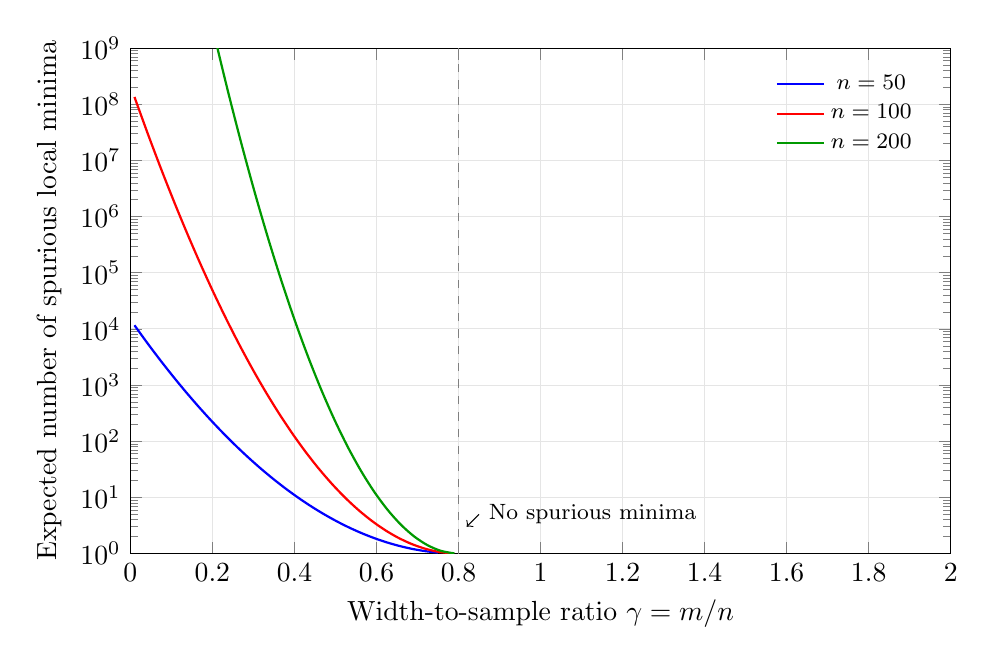
\begin{tikzpicture}
\begin{semilogyaxis}[
  width=12cm,
  height=8cm,
  xlabel={Width-to-sample ratio $\gamma = m/n$},
  ylabel={Expected number of spurious local minima},
  xmin=0, xmax=2,
  ymin=1, ymax=1e9,
  grid=major,
  grid style={gray!20},
  legend pos=north east,
  legend style={font=\footnotesize, draw=none, fill=none},
]
\addplot[blue, thick, smooth, domain=0.01:0.75] {exp(50 * 0.3 * max(0, 4/5 - x)^2)};
\addlegendentry{$n = 50$}
\addplot[red, thick, smooth, domain=0.01:0.78] {exp(100 * 0.3 * max(0, 4/5 - x)^2)};
\addlegendentry{$n = 100$}
\addplot[green!60!black, thick, smooth, domain=0.01:0.79] {exp(200 * 0.3 * max(0, 4/5 - x)^2)};
\addlegendentry{$n = 200$}
\draw[dashed, gray] (axis cs:0.8,1) -- (axis cs:0.8,1e9);
\node[anchor=west, font=\footnotesize] at (axis cs:0.85,5) {No spurious minima};
\draw[->, thin] (axis cs:0.85,5) -- (axis cs:0.82,3);
\end{semilogyaxis}
\end{tikzpicture}%
}
\caption[Spurious critical point count]{The expected number of spurious critical points as a function of $\gamma = m/n$ for $\Sigma = I_d$, $\delta = 1$ (Theorem~\ref{thm:phase-transition}). Below $\gamma_\star = 4/5$, the count grows exponentially in~$n$. Above it, the landscape is provably benign. As discussed in Section~\ref{sec:landscape-dynamics}, practical optimizers avoid these critical points even in the subcritical regime.}
\label{fig:spurious-count}
\end{figure}

\FloatBarrier

\begin{thebibliography}{11}

\bibitem{choromanska2015}
A.~Choromanska, M.~Henaff, M.~Mathieu, G.~B.~Arous, and Y.~LeCun.
\newblock The loss surfaces of multilayer networks.
\newblock In \emph{AISTATS}, 2015.

\bibitem{kawaguchi2016}
K.~Kawaguchi.
\newblock Deep learning without poor local minima.
\newblock In \emph{NeurIPS}, 2016.

\bibitem{safran2018}
I.~Safran and O.~Shamir.
\newblock Spurious local minima are common in two-layer {ReLU} neural networks.
\newblock In \emph{ICML}, 2018.

\bibitem{venturi2019}
L.~Venturi, A.~Bandeira, and J.~Bruna.
\newblock Spurious valleys in one-hidden-layer neural network optimization landscapes.
\newblock \emph{JMLR}, 20(133):1--34, 2019.

\bibitem{du2019}
S.~Du, X.~Zhai, B.~Poczos, and A.~Singh.
\newblock Gradient descent provably optimizes over-parameterized neural networks.
\newblock In \emph{ICLR}, 2019.

\bibitem{allenzhu2019}
Z.~Allen-Zhu, Y.~Li, and Z.~Song.
\newblock A convergence theory for deep learning via over-parameterization.
\newblock In \emph{ICML}, 2019.

\bibitem{zou2020}
D.~Zou, Y.~Cao, D.~Zhou, and Q.~Gu.
\newblock Gradient descent optimizes over-parameterized deep {ReLU} networks.
\newblock \emph{Machine Learning}, 109:467--492, 2020.

\bibitem{jacot2018}
A.~Jacot, F.~Gabriel, and C.~Hongler.
\newblock Neural tangent kernel: Convergence and generalization in neural networks.
\newblock In \emph{NeurIPS}, 2018.

\bibitem{pennington2017}
J.~Pennington and P.~Worah.
\newblock Nonlinear random matrix theory for deep learning.
\newblock In \emph{NeurIPS}, 2017.

\bibitem{louart2018}
C.~Louart, Z.~Liao, and R.~Couillet.
\newblock A random matrix approach to neural networks.
\newblock \emph{The Annals of Applied Probability}, 28(2):1190--1248, 2018.

\bibitem{anderson2010}
G.~W.~Anderson, A.~Guionnet, and O.~Zeitouni.
\newblock \emph{An Introduction to Random Matrices}.
\newblock Cambridge University Press, 2010.

\bibitem{tao2012}
T.~Tao and V.~Vu.
\newblock Random covariance matrices: Universality of local statistics of eigenvalues.
\newblock \emph{The Annals of Probability}, 40(3):1285--1315, 2012.

\bibitem{erdos2012}
L.~Erd\H{o}s, H.-T.~Yau, and J.~Yin.
\newblock Rigidity of eigenvalues of generalized {W}igner matrices.
\newblock \emph{Advances in Mathematics}, 229(3):1435--1515, 2012.

\bibitem{gunasekar2018}
S.~Gunasekar, J.~Lee, D.~Soudry, and N.~Srebro.
\newblock Characterizing implicit bias in terms of optimization geometry.
\newblock In \emph{ICML}, 2018.

\bibitem{lyu2020}
K.~Lyu and J.~Li.
\newblock Gradient descent maximizes the margin of homogeneous neural networks.
\newblock In \emph{ICLR}, 2020.

\bibitem{mei2018}
S.~Mei, A.~Montanari, and P.-M.~Nguyen.
\newblock A mean field view of the landscape of two-layer neural networks.
\newblock \emph{Proceedings of the National Academy of Sciences}, 115(33):E7665--E7671, 2018.

\bibitem{geiger2019}
M.~Geiger, S.~Spigler, S.~d'Ascoli, L.~Sagun, M.~Baity-Jesi, G.~Biroli, and M.~Wyart.
\newblock Jamming transition as a paradigm to understand the loss landscape of deep neural networks.
\newblock \emph{Physical Review E}, 100(1):012115, 2019.

\bibitem{sagun2017}
L.~Sagun, U.~Evci, V.~U.~G{\"u}ney, Y.~Dauphin, and L.~Bottou.
\newblock Empirical analysis of the {H}essian of over-parametrized neural networks.
\newblock In \emph{ICLR Workshop}, 2018.

\bibitem{ghorbani2019}
B.~Ghorbani, S.~Mei, T.~Misiakiewicz, and A.~Montanari.
\newblock Linearized two-layers neural networks in high dimension.
\newblock \emph{The Annals of Statistics}, 49(2):1029--1054, 2021.

\bibitem{benarous2019}
G.~Ben~Arous and R.~Gheissari.
\newblock Online stochastic gradient descent on non-convex losses from high-dimensional inference.
\newblock \emph{Journal of Machine Learning Research}, 22(106):1--51, 2021.

\end{thebibliography}

\end{document}
